\documentclass[12pt,a4paper]{article}
\usepackage[utf8]{inputenc}
\usepackage[T1]{fontenc}
\usepackage[ngerman]{babel}
\usepackage{amsmath}
\usepackage{amsfonts}
\usepackage{amssymb}
\usepackage{lmodern}
\usepackage{tikz-uml}
\usepackage[singlelinecheck=off, list=off]{caption}
\usepackage{enumitem}
\usepackage[backend=bibtex]{biblatex} 
\usepackage{float}
\makeatletter
\def\blx@maxline{77}
\makeatother
\addbibresource{literatur.bib}
\usepackage[colorlinks,bookmarksopen]{hyperref}

\newcommand*{\Title}{Projektseminar: Gestensteuerung einer 3D-Anwendung mittels Kinect}
\newcommand{\Authors}{Mario Janke,\\Peter Lindner,\\Patrick Stäblein}
\title{\Title}
\author{
	Mario Janke\\
	Peter Lindner\\
	Patrick Stäblein}
\date{}

\usepackage{fancyhdr}
\usepackage{vmargin}
\usepackage{setspace}
\onehalfspacing
\pagestyle{fancy}  %lustige fuß- und kopfzeilen
\parindent 0pt	
\parskip 0pt %
\emergencystretch 20pt
\setmarginsrb{3.0cm}{2.5cm}{2.5cm}{1.5cm}%  %ränder links oben rechts unten
             {1.0cm}{1.5cm}{1.0cm}{1.7cm}%  %kopf und fußzeile, höhe, abstand
\setlength{\leftmargin}{3.0cm}
\setlength{\textwidth}{15.5cm}
\setlength{\headwidth}{15.5cm}
\setlength{\topmargin}{2.0cm}
\lfoot{\footnotesize{\emph{\Title}}}
\cfoot{}
\rfoot{\footnotesize{\emph{\thepage}}}
\rhead{\emph{\leftmark}}
\chead{}
\lhead{}
\renewcommand{\footrulewidth}{0.5pt}
\renewcommand{\headrulewidth}{0.5pt}

\begin{document}
\begin{titlepage}
\setmarginsrb{2.5cm}{2.5cm}{2.5cm}{2.5cm}%  %ränder links oben rechts unten
             {1.0cm}{1.0cm}{1.0cm}{1.7cm}%  %kopf und fußzeile, höhe, abstand
\begin{center}
\vspace*{-2cm}
\includegraphics[width=.4\textwidth]{pictures/logo.jpg}\par 
\vspace*{1cm}{\small
Technische Universität Ilmenau\\
Fakultät für Informatik und Automatisierung\\
Institut für Praktische Informatik und Medieninformatik\\
Fachgebiet Graphische Datenverarbeitung}\par
\vfill
{\large Projektseminar}\par
\vspace*{.5cm}
%\rule{.9\textwidth}{4pt}\\[4ex]
{\huge\bfseries Gestensteuerung einer 3D-Anwendung mittels Kinect}\\[2ex]
%\rule{.9\textwidth}{4pt}\par
\vfill
\begin{tabular}{r l}
\emph{Autoren:}	& Mario Janke\\
	& Peter Lindner\\
	& Patrick Stäblein\\
&\\
\emph{Betreuer:} & M.\,sc. Julian Meder
\end{tabular}\par
\vfill
{\today}\par
\end{center}
\end{titlepage}
\tableofcontents
\clearpage
\section{Rahmenbedingungen}
Die vorliegende Ausarbeitung entstand im Rahmen des Projektseminars im Master-Studiengang Informatik an der Technischen Universität Ilmenau. Ziel und Zweck des Projektseminars ist die teambasierte Auseinandersetzung mit einem Forschungsgegenstand unter Verwendung von Fachliteratur.\par
Im Folgenden erläutern wir die Grundgegebenheiten, formulieren die uns gegebene Aufgabenstellungen und führen das titelgebende Tracking-System Microsoft Kinect ein.
	\subsection{Grundlagen und Motivation}\label{sec:grundl}
Gegeben ist eine bereits vorhandene 3D-Anwendung, die vom Betreuer des Projektseminars, Herrn M.\,Sc. Julian Meder, erstellt wurde. Das Programm wird zu Demonstrationszwecken z.\,B. am Tag der offenen Tür in den Räumlichkeiten des Fachgebiets genutzt. Innerhalb der Anwendung ist es möglich,
\begin{itemize}
\item ein Objekt zu laden und anzeigen zu lassen sowie 
\item die Kamera (bzw. Kameras) zu bewegen, zu rotieren und zu zoomen.
\end{itemize}
In Erweiterung soll das Programm auch andere Aufgaben der Objektmanipulation wahrnehmen können, insbesondere das Laden von mehreren Objekten in die Szene und eine abwechselnde Manipulation dieser im Sinne von Translation, Rotation, Skalierung und Löschung.\par
Um den oben genannten Demonstrationszweck zu erfüllen, ist das Programm auf einem Rechner im Laborraum verfügbar. Es rendert zwei Ausgabefenster aus zwei verschiedenen, stereoskopisch angeordneten Kamerasichten. Der Laborrechner ist per HDMI an einen 3D-Kameraaufbau angeschlossen, der aus zwei Projektoren im Nebenraum besteht. Sie werfen die beiden Ansichten aus dem Programm von hinten auf einen Projektionsschirm, der in die Trennwand von Labor- und Nebenraum eingelassen ist. Mittels handelsüblicher aus 3D-Kinos bekannten Shutterbrillen können Benutzer und Zuschauer sodann den 3D-Eindruck wahrnehmen.\par
Der konkrete Präsentationsablauf, wie er vor dem Projektseminar stattfand, lässt sich wie folgt skizzieren. Ein Vorführender befindet sich mit einigen Personen Publikum im Laborraum. Während er etwa sich und das Fachgebiet vorstellt, werden das Programm auf dem Laborrechner und die Projektoren gestartet. Am Rechner kann der Präsentierende dann z.\,B. ein Objekt laden. Diese Eingaben erfolgen per Maus und Tastatur.\par Anschließend kann er wieder vor die Zuhörenden treten, da die Kameramanipulationen, die das Programm erlaubt, auch mittels eines Präsentationspointers durchgeführt werden können. So kann er das Programm, während er vorträgt, bedienen. An die Zuhörer werden die genannten Shutterbrillen verteilt, sodass sie im Laufe des Vortrages ein 3D-Bild der Szene und der Manipulationen des Vortragenden sehen können.\par
In dieser Form hat der Ablauf Schwächen, die die Motivation für das Projektseminar bilden:
\begin{itemize}
	\item Die Steuerungen per Tastatur und Maus und noch stärker sogar die per Präsentationspointer bieten nur ein geringes Maß an Immersion.
	\item Es ist am Fachgebiet Technik (genauer Tracking-Systeme) vorhanden, mittels derer man eine Gestensteuerung für das genannte Programm realisiert werden kann. Eine solche ist für einen Vortrag wie etwa im Rahmen eines Tages der offenen Tür zusätzlich attraktiver für die Zuhörer und bietet außerdem dem Vortragenen ein weiteres Thema, auf das er eingehen und welches präsentiert werden kann.
\end{itemize}
Darüber hinaus motivierend ist auch die bloße Auseinandersetzung mit der genannten vorhandenen, aber bislang ungenutzten Technik und eine allgemeinere Untersuchung der Möglichkeiten, sie zielführend einzusetzen.
	\subsection{Aufgabenstellung}\label{sec:aufg}
Aus der in Abschnitt \ref{sec:grundl} genannten Motivation heraus, ist es Ziel des Projektes, die Steuerung der gegebenen 3D-Anwendung hinsichtlich ihrer Präsentation vor einer Zuschauergruppe zu erleichtern und intuitiv zu gestalten. Dabei wird besonderer Wert auf das Eintauchen des Vorführenden in die 3D-Szene gelegt. Diese Anforderung soll durch die Implementierung einer Gestensteuerung erfüllt werden. Nebenbei findet Arbeit mit den noch nicht eingesetzten Tracking-Systemen des Fachgebiets statt, die zukünftige Themen für studentische Arbeiten oder Forschung am Fachgebiet stützen kann. Die vorhandenen Trackingsysteme sind
\begin{itemize}
\item ein professionelles Motion-Capture-Trackingsystem zum Tracken von Raumpunkten über angebrachte Marker und Wands und
\item die Microsoft Kinect 2 zur optischen Gestenerkennung, i.\,W. mittels Kameraaufnahmen einer Infrarotprojektion.
\end{itemize}
Das so ausgewählte Trackingsystem ist also zur Implementierung einer Gestensteuerung der gegebenen Anwendung zu verwenden. Die dafür entwickelte Software soll folgendes leisten:
\begin{itemize}
\item Es soll in der Lage sein, sämtliche Steuerung und Manipulation, die oben beschrieben wurde, durchzuführen, d.\,h. Kamera und Objekte verschieben und drehen können.
\item Die Bedienung soll intuitiv und einfach sein, d.\,h. etwaige Gesten müssen bezüglich der ihnen zugeordneten Aktion einleuchtend und leicht ausführbar sein.
\item Die Steuerung soll ihrem Zweck angemessen genau sein, bestenfalls als glatte 1-zu-1-Übertragung von Handbewegungen auf die Szene.
\item Das entstehende Programm soll möglichst einfach eingebunden und wiederverwendet werden können.
\item Darüber hinaus soll eine Mastererkennung bzw. -verwaltung implementiert sein, d.\,h. ein Verfahren, das garantiert, dass auch nur die dafür vorgesehene Person das Programm steuert und niemand sonst. Hiermit wird ausgeschlossen, dass ein Fremder die Kontrolle über das Programm gewinnen kann und die Vorführung damit -- gewollt oder unbewusst -- behindert. Die als Vorführender ausgezeichnete Person soll auch später wieder erkannt werden können und die Kontrolle wiedererlangen, etwa nachdem sie einen Augenblick lang nicht im von der Kamera abgedeckten Bereich war.
\end{itemize}
Damit ist die vollständige Liste der Anforderungen gegeben und wird hier zur Übersicht nochmals im Kern zusammengefasst:\par\medskip
Ziel ist die Entwicklung einer Software
\begin{itemize}
\item unter Verwendung vorhandener Technik (einem Trackingsystem),
\item die eine Gestensteuerung der gegebenen Anwendung ermöglicht und 
\item dabei nur dem Präsentierenden als ausgezeichneter Person die Steuerung erlaubt.
\end{itemize}
Zur Umsetzung dessen fiel die Wahl auf die Microsoft Kinect 2 als Trackingsystem. Dies hatte vielerlei Gründe:
\begin{itemize}
\item Wegen ihrer kommerziellen Herkunft aus der Spieleindustrie (vgl. Abschnitt \ref{sec:kinect}) kann davon ausgegangen werden, dass sie bereits einem breiteren Publikum bekannt ist und gegebenenfalls auch besonders reizvoll erscheint.
\item Vom Verfahren der 3D-Daten-Gewinnung her (Genaueres in Abschnitt \ref{sec:kinect}) kann die Kinect vom Nutzer direkt und ohne weiterführende Vorbereitungsmaßnahmen verwendet werden. Markerbasierte Trackingsysteme haben diesen \glqq{}Plug-and-Play\grqq{}-Vorteil nicht.
\item Ähnlich zum ersten Punkt liegt hinsichtlich der Kinect aufgrund ihres Bekanntheitsgrades eine sehr gute Quellenlage im Internet vor. Sie verfügt über eine offizielle (wenn auch in Teilen knappe) Online-Dokumentation und da sie mit SDK und API veröffentlicht wurde, finden sich auch in einem breiteren Rahmen zahlreiche Lösungsdiskussionen und -präsentationen von Nutzern im Netz.
\end{itemize}

	\subsection{Trackingsystem Microsot Kinect}\label{sec:kinect}
\vspace*{-.8cm}
\begin{figure}[H]
\centering
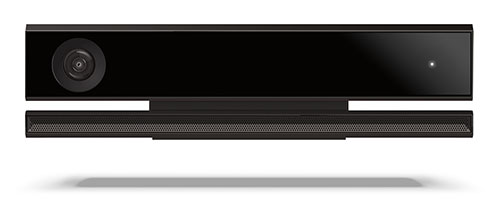
\includegraphics[width=.9\textwidth]{pictures/kinectimg.jpg}
\vspace*{-.5cm}
\caption{Frontalansicht der Kinect v2, Quelle: \cite{kinectimg}.}
\end{figure}
Die Kinect wurde in Versin 1 das erste Mal auf der E3 2009 in Los Angeles präsentiert, damals noch unter dem Namen \glqq{}Project Natal\grqq{} (siehe \cite{latimes}). Ziel war es, für Spiele der Xbox-Konsole von Microsoft den herkömmlichen Controller durch den Einsatz des gesamten Spielerkörpers zu ersetzen, nicht zuletzt, um damit ein breiteres Zielpublikum anzusprechen. Bereits zu diesem Zeitpunkt war geplant, unabhängigen Entwicklern die Verwendung und Programmierung des Systems zu ermöglichen (s. ebd.).\par 
Im Folgenden werden die technischen Spezifikationen der Kinect in ihrer aktuellen Version erläutert. Diese sind \cite{specs} entnommen. Die Kinect verfügt über eine Full-HD-Farbkamera und eine Infrarotkamera, die die Aufgabe des Tiefensensors erfüllt. Dieser ist mit 512 zu 424 Pixeln deutlich geringer aufgelöst. Der effektive Bereich ist laut Hersteller in einer Entfernung zwischen einem halben und 4,5 Metern. Die Kameras der Kinect liefern weiterhin maximal 30 Frames pro Sekunde. Weiterhin besitzt die Kinect ein Multi-Array-Mikrofon, mit dem Klang nicht nur aufgenommen, sondern auch hinsichtlich seiner Ausbreitung untersucht werden kann. Im Vergleich zu ihrer Vorgängerversion wurden vorwiegend Genauigkeitsverbesserungen vorgenommen, es kommt zu weniger Grundrauschen und die Objekterkennung ist generell stabiler und zuverlässiger. Mit der aktuellen Version können die Skelette von bis zu sechs Personen bei 25 Gelenkpunkten pro person vollständig getrackt werden (siehe Abbildung \ref{fig:Bild1}). Die zur Verfügung stehenden Gelenkpunkte lassen sich über die API des Kinect-SDK abfragen.
\begin{figure}[H] 
  \centering
  \begin{subfigure}{.6\textwidth}
  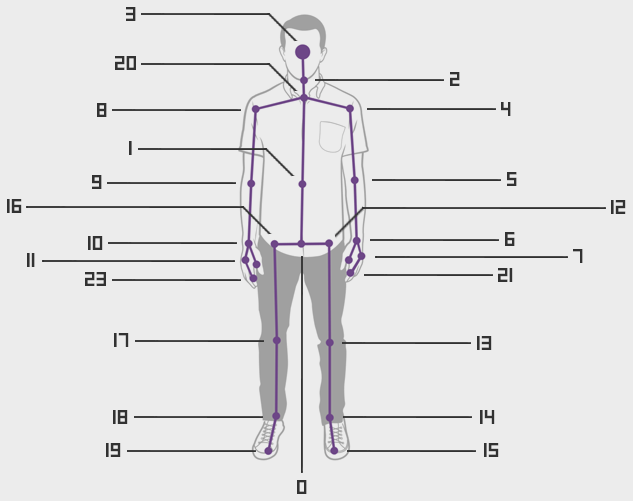
\includegraphics[width=\linewidth]{pictures/kinectskeleton-map2-1.png}
  \end{subfigure}\hfill
  \begin{subfigure}{.38\textwidth}
  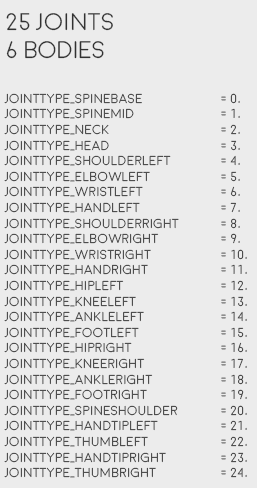
\includegraphics[width=\linewidth]{pictures/kinectskeleton-map2-2.png}
  \end{subfigure}
  \caption{\glqq{}Kinect V2 Joint ID Map\grqq{}, Gelenkpunkte die mit der Kinect getrackt werden können. Quelle (Ausschnitt): \cite{tracking2}}
  \label{fig:Bild1}
\end{figure}
Um die Tiefeninformation zu gewinnen, verwendet die Kinect in der zweiten Version ein sogenanntes Time-Of-Flight-Verfahren (hier und im Folgenden vgl. \cite{heise}). Grundlage ist die Gewinnung von 3D-Daten aus einem Kamerabild (in diesem Falle dem des Tiefensensors). Beim Time-Of-Flight-Verfahren wird für das ausgesendete Infrarotlicht gemessen, wie lange es braucht, um von der Objektoberfläche reflektiert zu werden und zurück zum Sensor zu gelangen. Beim Vorgänger, der Kinect-Version 1, wurde noch eine pseudorandomisiertes Muster auf die Szene projiziert und die Tiefeninformation daraus trianguliert (siehe \cite{gamasutra}). Ein Problem dieses Verfahrens ist die Forderung, für einen Punkt des Musters auch stets eine kleine Umgebung zu sehen, in der genug andere Lichtpunkte liegen, um eine Identifikation vorzunehmen. Der Time-Of-Flight-Ansatz der Kinect 2 besitzt diese Abhängigkeit nicht mehr. Eine weitere Verbesserung gegenüber der Kinect 1 ist das Vorhandensein eines eingebauten Umgebungslichtfilters: Wird ein Pixel von zu viel Licht aus dem sichtbaren Spektrum, insbesondere dem infrarotnahen Teil, getroffen, kann er während der Bestimmung zurückgesetzt werden (vgl. ebd.).\par 
Neben dem oben erwähnten, aus 25 Gelenkpunkte bestehenden und damit recht grobgranularen Skelett, dass die Kinect den Körpern zuweist, gibt es weiterhin für beide Hände einer getrackten Person einen \glqq{}Handzustand\grqq{}, der \glqq{}offen\grqq{}, \glqq{}geschlossen\grqq{}, \glqq{}unbekannt\grqq{} oder \glqq{}Lasso\grqq{} sein kann. Die Lassogeste besteht dabei aus einer halbgeschlossenen Hand, etwa mit zwei ausgestreckten Fingern).\par
Über eigene Konfidenzmechanismen, die dem Programmierer gegenüber transparent sind , verfügt die API nicht. In diesem Zusammenhang unterscheidet die Kinect, wie der Dokumentation \cite{trackingstate} auch zu entnehmen ist, nur zwischen drei Erkennungsgüten:
\begin{enumerate}
\item Ungetrackt: Das betroffene Gelenk wurde im Aufnahmebereich der Kinect nicht erkannt, es liegen keine Daten vor.
\item Gefolgert: Das betroffene Gelenk wurde nicht direkt erkannt, seine Daten jedoch aus den Restdaten angenähert. Über die Güte der Annäherung gibt es keinerlei Garantie.
\item Getrackt: Das Gelenk ist im Aufnahmebereich gefunden und getrackt und die Daten können als zuverlässig angesehen werden.
\end{enumerate}
Die Kinect-Eigenschaften hinsichtlich der Datengüte werden im Rahmen der Besprechungen zur Robustifizierung des Projektcodes zusätzlich und präziser in Abschnitt \ref{sec:robustheit} diskutiert.
Die hier aufgeführten Daten können über die Kinect-API abgegriffen werden. Dazu muss auf dem entsprechenden Rechner das Kinect-SDK vorliegen und die Kinect mit vorhandenen Treibern per USB und HDMI angeschlossen sein.\par 
In ihrer Erscheinungszeit kostete die Kinect v2 für Windows ca. 200 Euro, was verglichen mit professionellen 3D-Erfassungssensoren (die z.\,T. dasselbe Verfahren verwenden) ein niedriger Preis ist (vgl. \cite{heise}). Gerade aus diesem Grund und wegen der Verbreitung sind weitere Anwendungen aus Sicht der Forschung interessant, z.\,B. die Verwendung bei Assistenzrobotern (siehe \cite{thermalsens} und \cite{appearance}).\par 
	%
	%
\clearpage
\section{Vorüberlegungen}
	\input{sections/vorüberlegungen}
	%
	%
\clearpage
\section{Entwurfsentscheidungen}
	\subsection{Der Master}
	Der Master ist die Person (unter den getrackten Personen), der es obliegt, die Anwendung zu steuern, d.\,h. in unserem Anwendungsfall der Präsentation ist der Master der Präsentierende.
	Es muss gewährleistet werden, dass nur der Master das Programm steuert und dabei von weiteren Personen im Raum nicht (bzw. nicht ohne weiteres) gestört werden kann. Die Erkennung muss robust gegen Jittering der Kinectdaten sein.\par
\subsubsection{Möglichkeiten der Master-Identifikation}
	Grundsätzlich kamen für die Festlegung des Masters zwei Ideen auf. Zunächst sollte bei jedem Frame die getrackte Person identifiziert werden, die der Kinect bzgl. der z-Koordinate am nähesten ist und diese als Master festgelegt werden. Der Master könnte hierbei bei jedem Frame zwischen den getrackten Personen wechseln. \par
	Die zweite Möglichkeit war die Festlegung des Masters auf eine bestimmte Person, von der zunächst bestimmte Identifikations-Merkmale eingespeichert werden und die dann anhand dieser als Master reidentifiziert werden kann. Sofern diese Festlegung erst einmal geschehen ist, bleibt diese Person Master, selbst nachdem sich diese zwischenzeitlich in einem ungetrackten Zustand (beispielsweise beim Herausgehen aus dem getrackten Bereich) befunden hat und dann wieder als getrackt erkannt wird. Bei einer Recherche, welche Merkmale sich aus den von der Kinect gelieferten Daten extrahieren lassen ließen, um hierfür in Frage zu kommen, stießen wir hierbei auf verschiedene Möglichkeiten, von denen einige jedoch aufgrund ihrer Unpraktikabilität ausschieden (Erkennung anhand des Gangs oder anhand der Stimme würde bei unserer Anwendung keinen Sinn ergeben, da die Master-Person während der Bedienung kaum umher läuft und diese hierfür nicht zu sprechen braucht). Schließlich stießen wir auch auf Verfahren, die die Skelettdaten der Kinect zur Identifikation nutzen. Dies schien die für unsere Zwecke praktikabelste Lösung zu sein, wenngleich unser Ansatz die Skelettdaten zu nutzen im Vergleich zu denjenigen in den gefundenen Arbeiten stark vereinfacht wurde.\par
	Grundlegendstes Prinzip für die Identifizierung einer Person ist hierbei das Auslesen der Skelettkoordinatenpunkte mit Hilfe des Kinect SDKs und daraus der Ermittlung diverser Längen als Körperproportionen mittels der Berechnung des euklidischen Abstands zwischen den entsprechenden Skelettpunkten. Beispielsweise wird die rechte Oberarmlänge als Abstand zwischen dem rechten Schulterpunkt und dem rechten Ellenbogenpunkt ermittelt. Weitere Körperproportionen die verwendet wurden sind unter anderem die Schulterbreite, Hüftbreite, Unterarmlänge, Abstand zwischen Hals und Kopf. \par

\subsubsection{Robustheit}
Nach einigen Experimenten mit den Körperproportionen wurde festgestellt, dass einige Proportionen übermäßig große Abweichungen aufwiesen, wenn die gleiche Person in unterschiedlichen Posen mit der Kinect vermessen wurde bzw. dass sich einige Skelettpunkte \glqq{}verschieben\grqq{}, wenn man mit einem Körperteil darüber fährt. (Beispielsweise die gemessene Schulterbreite, welche sich signifikant zwischen der Standard-Pose und einer Pose bei der die Arme über den Kopf gestreckt sind unterschied.) 
\begin{figure}[h!]
		\centering
		\includegraphics[width=.8\textwidth]{pictures/standardpose_.png}
		\caption{Die Standardpose, in der sich eine Person befinden muss, damit sie vermessen werden kann.}\label{fig:standardp}
		\end{figure}
Aus diesem Grund wird die Vermessung einer Person nur durchgeführt, wenn sich die entsprechende Person über eine bestimmte Anzahl von Frames (etwa 20) durchgehend in der festgelegten Standard-Pose befindet. Falls während der Sammlung das Einhalten der Standard-Pose unterbrochen wird, wird die Sammlung erneut begonnen.\par
Ein weiteres Problem, das zu lösen war bestand darin, dass selbst beim Stillhalten, jedoch hauptsächlich bei der Bewegung einer getrackten Person, Skelettpunkte kurzzeitig auf einen anderen weiter entfernten Raumpunkt springen konnten, was teils zu unrealistischen Messungen einer Körperproportion für einzelne Frames führte (z.B. Messung einer Oberarmlänge von 2 Metern). Um derartige Ausreißer zu eliminieren wird der während der Vermessung einer Person zur Einspeicherung als Master über mehrere Frames der Mittelwert sowie die Standardabweichung jeder Körperproportion berechnet und jeder Wert der nicht innerhalb des Intervalls um den Mittelwert mit der Ausdehnung der Standardabweichung liegt, d.h. des Intervalls \[(\text{Mittelwert}-\text{Standardabweichung}\cdot \text{Faktor}, \text{Mittelwert}+\text{Standardabweichung}\cdot \text{Faktor})\text,\] ignoriert. 
\par
Weiterhin wird darauf geachtet, dass alle für die Vermessung relevanten Körperproportionen mit ausreichender Konfidenz von der Kinect getrackt werden. Die Kinect liefert hierfür für jeden Skelettpunkt einen von drei möglichen Konfidenzwerten, der angibt, wie wahrscheinlich die von der Kinect gelieferte Koordinatenwerte für diesen Punkt dem tatsächlichem Wert entsprechen. (Die drei Konfidenzwerte heißen Tracked, Inferred, NotTracked; wobei Tracked die höchste Konfidenz und NotTracked die niedrigste Konfidenz für einen Skelettpunkt bezeichnet). Ist in einem Frame der Konfidenzwert von einem der beiden Skelettpunkte, aus denen eine Körperproportion berechnet wird, nicht Tracked, so wird diese Körperproportion für diesen Frame nicht berücksichtigt bzw. mit Null gewichtet. \par
\subsubsection{Umsetzung}
Eingebettet in unsere Hauptschleife geht die Master-Identifikation folgendermaßen von statten: Beim Start des Programms ist zunächst einmal die Person Master, die bzgl. der Kinect die geringste z-Koordinate aufweist. Hierfür wird bei jedem Schleifendurchlauf abgefragt, welche der 6 (potenziell) getrackten Personen, den geringsten z-Wert hat. Der Master wird somit bei jedem Frame neu bestimmt.
\par
 Durch die Betätigung einer vorher festgelegten Taste wird schließlich die Master-Festlegung auf eine bestimmte Person aktiviert. Hierzu werden die Körperproportionen der Person, die als erstes in Standardpose erkannt wird, über mehrere Frames aus den Skelettdaten extrahiert, gepuffert und schließlich aus diesen für jedes Körpermerkmal der Mittelwert sowie die Standardabweichung berechnet. (Sofern beim Tastendruck noch keine Person im getrackten Bereich war, wird gewartet bis eine Person getrackt wird und diese die Standard-Pose einnimmt.) Der Mittelwert und die Standardabweichung werden dazu verwendet Ausreißer zu identifizieren und zu entfernen, um schließlich die Mittelwerte erneut ohne die Ausreißer zu berechnen. Neben diesen Mittelwerten für die nun als Master festgelegte Person, wird außerdem die von der Kinect vergebene ID der Person eingespeichert. Diese bleibt dieser Person zugeordnet, solange sie durchgehend getrackt wird. Verlässt der Master den getrackten Bereich oder wird anderweitig vorübergehend nicht getrackt (beispielsweise wenn dieser von einer anderen Person verdeckt wird) und kommt danach wieder in den getrackten Bereich zurück, hat dieser eine neue ID. In diesem Fall muss der Master neu identifiziert werden. 
 
 \begin{figure}
\includegraphics[width=\textwidth]{pictures/sensors-16-01965-g005.jpg}
\caption{Neuzuordnung von IDs nach zwischenzeitlichem \glqq Verlust\grqq{} von Skeletten, Quelle:\cite{bodyprop}}
\label{fig:fehlerk}
\end{figure}
 \par
 Solange der Master noch nicht gefunden wurde, werden hierfür für jede Person, die in Standard-Pose erkannt wird, die Körperproportionen über eine gewisse Anzahl (etwa 20) an Frames mit denen der für den Master eingespeicherten Werte verglichen. Schließlich wird aus den frameweise berechneten Abweichungen der Durchschnitt berechnet. Ist diese durchschnittliche Abweichung kleiner als ein im Programm festgelegter Wert ist diese als Master identifiziert worden. Diese kann nun mit der Steuerung des Programms fortfahren.
	
	
	\subsection{Gesten und ihre Wirkung}\label{sec:gesten}
Für die eingangs erwähnte Aufgabenstellung war es notwendig, bestimmte Programmfunktionalitäten mit Gesten zu verbinden. Einerseits hätte die Möglichkeit bestanden, mit dem Kinect-eigenen Visual Gesture Builder Gesten aufzunehmen und einzulernen. Diese Gesten werden dann als Datenbank ins Programm geladen und bei Vorführung erkannt. Dies erspart natürlich primitive aber umständliche Low-Level-Erkennungsmechanismen. Weiterhin sind hierdurch einige weiterführende Möglichkeiten gegeben wie etwa die Rückgabe, bis zu welchem Punkt eine Geste bereits ausgeführt wurde (in Bezug zur Gesamtgeste, d.\,h. beispielsweise wieviel Prozent einer Armbewegung vordefinierte Länge bereits ausgeführt wurde). Anderseits wiederum können durch die Kinect-Rohdaten auch eigene Erkennmechanismen implementiert werden. Dies bietet dem Programmierer die vollständige Kontrolle und Freiheit darüber, wie er Gesten definiert und auswertet, statt wie im Falle des Gesture Builders auf ein gewisses Rahmenwerk angewiesen zu sein. Änderungen können kurzfristig und schnell vorgenommen werden und für einfache Projekte ist die Zusatzfunktionalität, die der Visual Gesture Builder gestattet nicht vonnöten, der eher für komplexere Gestenfolgen ausgelegt zu sein scheint. Demgegenüber ist für diese Direktimplementierung von Gesten aber die bereits erwähnte Low-Level-Erkennung zu implementieren, d.\,h. ein Extrahieren von Bewegungen und Bewegungsrichtungen aus den Skelett- und Gelenkdaten, die die Kinect bestimmt. Aus dieser Gegenüberstellung heraus, ist für den gegebenen Einsatzzweck eine direkte Gestenerkennung die sinnvollere Alternative. Mit dem Visual Gesture Builder ist es schlicht nicht möglich, eine wie beabsichtigte $1$"=zu"=$1$"=Abbildung zwischen Geste und Wirkung zu bewerkstelligen.\par 
	Auch bei der Low-Level-Erkennung gibt es jedoch verschiedene Ansätze bzw. Ausprägungen. Es ist sogar das Implementieren nicht ganz primitiver Gestenfolgen möglich, indem eine Geste zeitlich und räumlich in verschiedene Segmente unterteilt wird. Dies sei an einem Beispiel erläutert: Es soll eine Winkgeste der rechten Hand erkannt werden. Die Geste wird in zwei Segmente geteilt. Ein Wechsel zwischen den Segmenten findet statt, wenn die horizontale Position der Hand und des Ellenbogens wechseln. Wird dieser Übergang dreimal in Folge erkannt, so wurde die Winkgeste präsentiert.\par
	Eine genauere Auseinandersetzung mit der Aufgabenstellung und allgemeinen Vorstellungen von intuitiven Gesten für die zu realisierenden Funktionalitäten zeigte jedoch auf, dass auch eine Segmenteinteilung von Gesten für das Projekt nicht notwendig ist. Stattdessen sind die gegebenen Aufgaben (ein Verschieben oder Rotieren per Geste) in ihrer Struktur simpel genug, um die verschiedenen Wirkungen mit diskreten Gesten zu erzeugen, d.\,h. es genügt die Erkennung einer Geste durch bestimmte Zustände der Kinect-Rohdaten zu einem einzigen Zeitpunkt. Um die Wirkung jedoch zu erzielen, ist natürlich auch eine Betrachtung der Geste über mehrere Frames notwendig.\par\medskip
	Im Folgenden ist der im Projekt Verwendung findende Gestenkatalog erklärt. Dabei wird darauf eingegangen, was der Benutzer vorführen muss, damit die Geste erkannt wird und wie die Geste genutzt wird, um in der Anwendung die Kamera oder Objekte zu manipulieren:\par\bigskip
	\begin{description}
		\begin{figure}[H]
		\centering
		\includegraphics[width=.8\textwidth]{pictures/translate_.png}
		\caption{Die (Kamera-)Translations-Geste, mit und ohne eingezeichnetes Skelett und HandStates.}\label{fig:translateg}
		\end{figure}
		\item[TRANSLATE\_GESTURE] (siehe Abb. \ref{fig:translateg})\par
		Der Benutzer hat beide Hände geöffnet, mit den Handflächen zur Kamera (wichtig ist nur, dass die Kinect beide Hände als offen erkennt, die genaue Haltung ist dabei egal). Ein paralleles Verschieben der beiden Hände in eine Richtung bewirkt ein zur Bewegungsgeschwindigkeit proportionales Verschieben der Kamera in diese Richtung.\par 
		Wie in den Vorüberlegungen (Abschnitt \ref{sec:vor}) schon erwähnt ist dies eine einfache Übertragung des Prinzips nachdem eine Person in der Realität einen großen Gegenstand verschieben würde und wird daher der geforderten Intuitivität gerecht.
		\par
		\begin{figure}[H]
		\centering
		\includegraphics[width=.8\textwidth]{pictures/rotate_.png}
		\caption{Die (Kamera-)Rotations-Geste, mit und ohne eingezeichnetes Skelett und HandStates.}\label{fig:rotateg}
		\end{figure}		
		\item[ROTATE\_GESTURE] (siehe Abb. \ref{fig:rotateg})\par
		Der Benutzer hat beide Fäuste geballt. Dann bewirkt eine gleichzeitige Bewegung der Hände auf einer Kreisbahn eine Rotation der Kamera um die Senkrechte des zugehörigen Kreises.
		Analog zur Verschiebegeste fand diese Geste bereits in den Vorüberlegungen (Abschnitt \ref{sec:vor}) Erwähnung. Die Aufgabe, eine Rotation im Raum zu vollführen ist leider weniger alltäglich als die des Verschiebens von Gegenständen. Ein verwandtes Prinzip ist jedoch das des Lenkrades, das man sich --  ins Dreidimensionale erweitert -- als Lenkkugel vorstellen kann. Mittels der üblichen Lenkbewegung kann dann um beliebige Raumachsen rotiert werden. Ähnlich findet dies auch etwa bei der Bedienung von Münzfernrohren statt. Wegen dieser Analogien, kann davon ausgegangen werden, dass der Benutzer schnell ein intuitives Verständnis von der Wirkungsweise dieser Geste entwickelt.
		\par
		\begin{figure}[H]
		\centering
		\includegraphics[width=.8\textwidth]{pictures/grab_.png}
		\caption{Die Objektmanipulations-Geste, mit und ohne eingezeichnetes Skelett und HandStates.}\label{fig:grabg}
		\end{figure}
		\item[GRAB\_GESTURE] (siehe Abb. \ref{fig:grabg})\par
		Zunächst war angedacht, dass die Objektmanipulation dieselben Gesten verwendet wie die Kameramanipulation und die Unterscheidung, was manipuliert wird durch einen globalen Zustand gefällt wird. Bei näherer Betrachtung dieses Ansatzes und ersten Tests dessen fiel auf, dass es so schwierig ist, zwischen Kamera- und Objektmanipulation zu wechseln. Weiterhin schien es während des Testens weniger intuitiv als zuvor angenommen, ein Objekt auf diese Art und Weise zu manipulieren. Es bedarf hier also anderer Ansätze.\par 
		In das Problem der Objektmanipulation eingeschlossen ist das Problem des Object-Pickings, d.\,h. die Auswahl des zu manipulierenden Objekts vom Bildschirm. Auch dies wäre mit der oben beschriebenen Methode, die die Gesten der Kameramanipulation verwendet, nur schwierig und umständlich realisierbar gewesen. Das Object-Picking bietet jedoch einen anderen Weg, einen Ansatz für eine Objektmanipulationsgeste zu finden. Ein alltägliches und dem Benutzer bekanntes Beispiel hierfür ist das einfache Greifen nach einem Gegenstand -- dies motiviert auch den Namen \glqq{}GRAB\grqq{}-Geste. Übertragen in eine Geste ließe sich dies durch eine erhobene und geschlossene Hand definieren. In weiterer Analogie zum Alltagsbeispiel sollte ein Hin- und Herbewegen der Hand, mit der gegriffen wurde (der \glqq Kontroll-Hand\grqq{}) auch das Objekt hin"= und herbewegen. Die Rotation führt jedoch bei dieser Geste zu einem Problem: Mit der geschlossenen Hand ist die Erkennung der Orientierung des entsprechenden Gelenks durch die Kinect zu schlecht, um an dieser Stelle sinnvoll Verwendung zu finden. Im Programm äußerte sich dies einerseits durch ein Ausbleiben der Auswirkungen vorgeführter Rotationen, andererseits aber auch durch ein starkes Rauschen. Probleme dieser Art treten auch an anderer Stelle auf und sind behandelbar (dies wird in Abschnitt \ref{sec:robustheit} deutlich), hier jedoch wurden die Ergebnisse so schlecht, dass eine andere Gestendefinition nötig war. Die Ergebnisse wurden direkt deutlich besser, wenn die GRAB"=Geste durch eine gehobene und offene (!) Hand definiert wurde. Die größere Fläche bietet der Kinect mehr Anhaltspunkte und verbessert so die Genauigkeit für die Orientierung, etwa wenn die Handfläche gekippt bzw. gedreht ist.
		\par
		\begin{figure}[H]
		\centering
		\includegraphics[width=.8\textwidth]{pictures/fly_.png}
		\caption{Die Flug-Geste, mit und ohne eingezeichnetes Skelett und HandStates.}\label{fig:flyg}
		\end{figure}
		\item[FLY\_GESTURE] (siehe Abb. \ref{fig:flyg})\par
		Im Rahmen der Tests mit einem Beispielobjekt wurde schnell deutlich, dass es auch eine einfache Möglichkeit geben sollte, Bewegungen über etwas weitere Strecken durch den Raum zu vollführen, ohne dabei ständig zwischen dem Vorführen einer Geste und einem \glqq Nachgreifen\grqq{} wechseln zu müssen. Eine übliche Lösung für eine solche Aufgabe ist ein Flugmodus. Im konkreten Anwendungsfall sollte dann das Vorführen einer besonderen Geste bewirken, dass die Kamera losfährt und erst anhält, wenn die Geste nicht mehr präsentiert wird.\par 
		Die FLY"=Geste entspricht dem Ausstrecken beider Arme vor den Körper, sodass sich die Hände mehr oder weniger am selben Punkt im 3D"=Raum befinden. Passiv findet bei dieser Geste im Programm eine Bewegung nach vorne statt. Durch Schwenken der Arme soll der Nutzer dabei die Richtung der Bewegung beeinflussen können, d.\,h. ein Zeigen der Arme nach oben bewirkt, dass die Bewegung immer weiter nach oben gezogen wird, während mit einem Zeigen nach links oder rechts eine Kurve geflogen werden kann. Dabei bestimmt der Ausschlag der Arme beim Zeigen (verglichen mit der Ausgangsposition, in der beide Arme genau nach vorne gerichtet sind) die Stärke der Richtungsänderung. Um eine sogenannte Fassrolle durchzuführen oder sich \glqq{}in Kurven legen\grqq{} zu können, kann der Nutzer nebenbei seine Schulterpartie in die entsprechende Richtung kippen. Insgesamt ist die Steuerung des Flugmodus in ihrem Funktionsumfang damit ähnlich zu üblichen Steuerungen von Flugzeugen in Actionspielen oder Simulationen: Es findet eine automatische Bewegung nach vorne statt, die in verschiedene Achsen gekippt werden kann.\par
	Diese erneute Prinzipübertragung macht die Geste intuitiver. Mit Hilfe dieser Fluggeste hat der Benutzer eine im Gegensatzu zur Bewegung über Drehen und Schieben einfache Möglichkeit, sich etwa durch ein System von Gängen in einer 3D-Szene zu bewegen und generell Strecken zurückzulegen, statt Objekte zu betrachten. Werden die Strecken zu lang, kann diese Geste jedoch anstrengend für den Benutzer sein. Bei alternativen Anwendungen wäre dies zusätzlich zu bedenken und eine dem abweichenden Zweck besser angepasste Gestendefinition zu verwenden.
		\par		
		\item[UNKNOWN] Dies enthält alles, was als keine der anderen Gesten erkannt wird. Die Kamera und geladene Objekte sollen, solange diese Geste gezeigt wird, stillstehen.\par
		Neben der naheliegenden Motivation, dass der Nutzer die Szene gegebenenfalls auch bei Ruhe betrachten möchte, dient diese \glqq Geste\grqq{} (oder besser \glqq Nicht-Geste\grqq{}) darüber hinaus noch einem anderen Zweck. Sie kann in andere Gesten, wie beispielsweise Translationen, eingebaut werden, um diese aufzubrechen und \glqq nachgreifen\grqq{} zu können. Erst dies gestattet dem Nutzer, während der Bedienung an Ort und Stelle stehen bleiben zu können.
	\end{description}
	Die Verwendung der Gesten hat ergeben, dass es notwendig ist, bei derartig selbst implementierten Gesten auch eigene Robustheitsmechanismen einzubauen, die die Gestenerkennung gegen Schwankungen der Kinecterkennung (etwa des Status einer Hand) abhärten. Für genauere Informationen hierzu sei auf Abschnitt \ref{sec:robustheit} verwiesen.
	\subsection{Zustandsmaschine}
	Das Programm besteht aus zwei Grundmodi der Manipulation: Einerseits der Manipulation der Kamera und andererseits jener des Objekts. Wir können diese beide Modi als zwei Superzustände auffassen, innerhalb derer sich wiederum unterscheidet, auf welche Art und Weise wir manipulieren. Die Zustandsmaschine dient einerseits der Kapselung und Modularisierung der von uns bereitgestellten Funktionen und bildet andererseits die Struktur unserer Manipulationsmodi abstrakt ab.\par 
	Die Zustandsmaschine befindet sich zu jedem Zeitpunkt in einem Zustand. In diesem Zustand findet eine Berechnung der Parameter statt, die unser Programm zurückgibt, die wiederum die Manipulation beschreiben, die ausgeführt werden soll. Dies geschieht durch Auswertung der gesehenen Geste und die Berechnung entscheidender Größen, u.\,U. unter Einbeziehung der Werte vergangener Frames. Schließlich erfolgt basierend auf der präsentierten Geste ein Zustandswechsel am Ende eines Berechnungsschritts. Die Zustandsmaschine ist in Abb. \ref{fig:sm} zu sehen. Im Folgenden erklären wir die Zustände, ihre Semantik und die enthaltenen Berechnungen etwas näher:
	\begin{description}
		\item[IDLE] Dieser Zustand entspricht dem Initialzustand unserer Zustandsmachine. Er ist eine Art Default-Zustand, in dem keine Kamera- und auch keine Objektmanipulation (genauer: keine Berechnung überhaupt) vorgenommen wird. Der Zustand wird betreten, wenn keine der vordefinierten Gesten sicher genug erkannt wurde. Durch Ausführung der entsprechenden Gesten gelangt man zurück in die anderen Zustände.
		\item[CAMERA\_TRANSLATE] Dieser Zustand gehört zur Kameramanipulation. In ihm werden gemäß der oben erklärten Geste die Parameter zur Kamerabewegung bestimmt. Ziel ist die direkte Übertragung der Handbewegungen des Benutzers auf die Kamerabewegung, die im lokalen Raum der Kamera stattfindet. Wir berechnen dazu aus den gepufferten Positionswerten von linker und rechter Hand die diskrete Ableitung, die uns ein Maß für die Geschwindigkeit der Bewegung liefert. Ebenso erhält man daraus die Richtung, in die die Hände bewegt wurden. Die Geschwindigkeit wird dann mit der vergangenen Zeit zwischen dem aktuellen und dem vorhergehenden Frame multipliziert, um wieder einen Entfernungswert zu erhalten. Daraus entstehen die Translationsparameter für die $x$"=, $y$"= und $z$"=Richtungen, die für diesen Zustand unsere \texttt{motionParameters} definieren.
		\item[CAMERA\_ROTATE] Dieser Zustand gehört ebenfalls zur Kameramanipulation. Analog zu oben wird hier die Rotation vorbereitet. Die Rotation ist konzeptionell nahe in der Translation. Während die Geste aktiv ist, wird eine Achse zwischen linker und rechter Hand des Benutzers bestimmt. Bewegt der Benutzer die Hände, so verändert sich die Achse. Ein Quaternion, der die Achsen ineinander überführt, wird berechnet, und analog zur Translation als Geschwindigkeit interpretiert. Dieser proportional zur verstrichenen Zeit zum vorhergegangenen Frame verkleinert und auf die Kamerarotation angewandt.
		\item[OBJECT\_MANIPULATE] Die Objektmanipulation realisiert das einhändige Packen eines virtuellen Objektes mit einer einzigen Hand. Dabei werden Aspekte der Translation und Rotation abgewandelt verwendet. Die Bewegung der packenden Hand wird sehr ähnlich zur Kamera-Translation direkt übertragen. Im Gegensatz zu CAMERA\_TRANSLATE wird diese allerdings auf das Objekt angewandt. Außerdem soll jede Rotation der packenden Hand auf das Objekt übertragen werden. Dazu wird Kinect::JointOrientation genutzt, welches die Orientierung der Hand im Raum als Quaternion bereitstellt. Es wird eine Art Differenz zwischen der Orientierung eines Frames und den gepufferten Vorgängerorientierungen gebildet. Dies findet statt, indem die Vorgängerorientierungen invertiert auf die aktuelle Orientierung angewandt werden. Wie zuvor kann diese Differenz als Geschwindigkeit interpretiert werden. Bei der Anwendung auf das Objekt muss jedoch beachtet werden, dass eine Drehung der Hand beispielsweise um ihre Z-Achse nicht unweigerlich auch einer Drehung des Objektes um dessen Z-Achse haben soll. Für natürliches Verhalten muss die Rotation selbst noch abhängig von Objekt- sowie Kamerarotation gedreht werden.
		\item[FLY] Dieser Zustand wurde nachträglich eingeführt, als die Notwendigkeit eines Flug-Modus deutlich wurde. Er wird mittels Vorführung der FLY"=Geste betreten und analog zu den anderen Zuständen verlassen. Der Flugmodus soll eine durchgehende Bewegung realisieren, ohne dass der Benutzer sich permanent bewegt. Sie bildet primär eine Alternative zum wiederholten Anwenden von CAMERA\_TRANSLATE. Während die Geste aktiv ist, wird eine Translation mit festen Werten nach vorn vorgenommen. Außerdem ist es möglich, durch die Neigung der nach vorn gestreckten Arme zu lenken. Dazu wird die mittlere Handposition mit einem Referenzpunkt auf dem Körper des Benutzers verglichen. Die Abweichung der Position von einer neutralen Ausgangsposition bestimmt die Lenkrichtung. Die Stärke der Auslenkung bestimmt dabei die Stärke der Rotation. Um schnellere Drehungen zu gewährleisten, werden starke Auslenkungen noch zusätzlich verstärkt. Analog zur CAMERA\_ROTATE wird ein Quaternion berechnet, welcher die neutrale Position auf die gegebene Position abbildet. Er wird wie üblich angewandt. Außerdem wird die Neigung der Achse von linker Schulter zu rechter Schulter bestimmt. Diese wird in eine kontinuierliche Seitwärtsrolle übersetzt.
	\end{description}
	Zur Verdeutlichung sei darauf hingewiesen, dass von jedem Zustand zu jedem anderen übergegangen werden kann, wobei dieser Übergang lediglich anhand erkannter Gesten erfolgt: Wird eine unserer Gesten erkannt (Details siehe Abschnitt \ref{sec:robustheit}), so wird der zugehörige Zustand betreten. Da unser Programm darauf ausgelegt ist, während des Event-Loops einer Hauptanwendung zu laufen, besteht die Zustandsmaschine ab ihres Starts permanent (bzw. bis zum Ende der Hauptanwendung) und besitzt keinen Finalzustand.\par
	Genaueres zum Aussehen der State-Machine als Datenstruktur ist in Abschnitt \ref{sec:ds} zu finden.
	\begin{figure}[h!]
	\centering
	\usetikzlibrary{positioning}
\resizebox{\textwidth}{!}{
\begin{tikzpicture}

%%IDLE-State
\umlbasicstate[x=8,y=4, name=IDLE, fill=white]{IDLE}

%%INIT-State
\umlstateinitial[below=2cm of IDLE.south, name=INIT]
	\umltrans{INIT}{IDLE}

%%Superstate Kamera-Manipulation
\begin{umlstate}[x=0,y=8,name=CAM, fill=black!20]{Kamera-Manipulation}
	%%%%%%%%%%%%%%
	%% Zustände %%
	%%%%%%%%%%%%%%
	%%Zustand Kamerabewegung
	\umlbasicstate[x=0,y=0, name=CAMTRANS, fill=white]{CAMERA\_TRANSLATE}
	%%Zustand Kameradrehung
	\umlbasicstate[x=0,y=-4, name=CAMROT, fill=white]{CAMERA\_ROTATE}
	%%Zustand FLY
	\umlbasicstate[x=0,y=-8, name=FLY, fill=white]{FLY}
	
	%%%%%%%%%%%%%%%%%%
	%% Transitionen %%
	%%%%%%%%%%%%%%%%%%
	%\umlHVHtrans[anchor1=20,anchor2=170,arg={ROT...},pos=1.5]{CAMTRANS}{CAMROT}
	%\umlHVHtrans[anchor1=-170,anchor2=-20,arg={TRA...},pos=1.5]{CAMROT}{CAMTRANS}
	
%	\umltrans[recursive=-120|-170|3cm, recursive direction=bottom to left, arg={TRANSLATE\_GESTURE},pos=1.3]{CAMTRANS}{CAMTRANS}
	%\umltrans[recursive=-10|-60|3cm, recursive direction=right to bottom, arg={ROTATE\_GESTURE},pos=2.6]{CAMROT}{CAMROT}
\end{umlstate}


%%Superstate Objekt-Manipulation
\begin{umlstate}[x=8,y=8,name=OBJ, fill=black!20]{Objekt-Manipulation}
	%%%%%%%%%%%%%%
	%% Zustände %%
	%%%%%%%%%%%%%%
	%%Zustand Kamerabewegung
	\umlbasicstate[y=0,name=OBJMAN, fill=white]{OBJECT\_MANIPULATE}
	%%%%%%%%%%%%%%%%%%
	%% Transitionen %%
	%%%%%%%%%%%%%%%%%%
	%\umltrans[recursive=-40|-140|2cm, recursive direction=bottom to bottom, arg={GRAB\_GESTURE},pos=1.5]{OBJMAN}{OBJMAN}
\end{umlstate}

\umltrans[recursive=-10|-60|3cm, recursive direction=right to bottom]{OBJMAN}{OBJMAN}
\umltrans{CAMROT}{OBJMAN}
\umltrans{FLY}{OBJMAN}
\umltrans[anchor1=110,anchor2=-110]{IDLE}{OBJMAN}
\umltrans{CAMTRANS}{OBJMAN}

\node at (4.6,8.6) {G};
\node at (5.2,6.6) {G};
\node at (5.8,6.5) {G};
\node at (7.4,6.5) {G};
\node at (11.7,7.6) {G};

\umltrans[recursive=-10|-60|3cm, recursive direction=right to bottom]{IDLE}{IDLE}
\umltrans{CAMROT}{IDLE}
\umltrans[anchor1=15,anchor2=-140]{FLY}{IDLE}
\umltrans{OBJMAN}{IDLE}
\umltrans{CAMTRANS}{IDLE}

\node at (8.3,5.6) {U};
\node at (9.7,4.4) {U};
\node at (6.4,4.8) {U};
\node at (6.1,4.6) {U};
\node at (7,3) {U};

\umltrans[recursive=-60|-120|1cm, recursive direction=bottom to bottom]{FLY}{FLY}
\umltrans{CAMROT}{FLY}
\umltrans{IDLE}{FLY}
\umltrans[anchor1=-120,anchor2=35]{OBJMAN}{FLY}
\umlHVHtrans[anchor1=-190,anchor2=-160,arm1=-2cm]{CAMTRANS}{FLY}

\node at (-1,-1.5) {F};
\node at (-1.5,-.5) {F};
\node at (0.4,1.7) {F};
\node at (2.5,2) {F};
\node at (2.2,1.6) {F};

\umltrans[recursive=-170|-190|.5cm, recursive direction=left to left]{CAMROT}{CAMROT}
\umltrans[anchor1=-110,anchor2=110]{CAMTRANS}{CAMROT}
\umltrans[anchor1=-163,anchor2=-10]{IDLE}{CAMROT}
\umltrans[anchor1=-160,anchor2=35]{OBJMAN}{CAMROT}
\umltrans[anchor1=110,anchor2=-110]{FLY}{CAMROT}

\node at (-.8,5.8) {R};
\node at (-.8,2.8) {R};
\node at (-2.6,5) {R};
\node at (1.3,5.8) {R};
\node at (2.6,3.7) {R};

\umltrans[recursive=-10|5|1cm, recursive direction=right to right]{CAMTRANS}{CAMTRANS}
\umltrans{CAMROT}{CAMTRANS}
\umltrans[anchor1=140,anchor2=-20]{IDLE}{CAMTRANS}
\umltrans[anchor1=-175,anchor2=-5]{OBJMAN}{CAMTRANS}
\umlHVHtrans[anchor1=-190,anchor2=-170,arm1=-3cm]{FLY}{CAMTRANS}

\node at (3.6,8.8) {T};
\node at (3.4,7.3) {T};
\node at (-3.4,7.4) {T};
\node at (.5,6.8) {T};
\node at (4,7.8) {T};

%\umlVHVtrans[arm1=-1cm,anchor1=-60,anchor2=-150,arg={GRAB\_GESTURE},pos=1.4]{IDLE}{OBJMAN}
%\umlVHVtrans[arm1=-2cm,anchor1=-30,anchor2=-120,arg={UNKNOWN\_GESTURE},pos=1.5]{OBJMAN}{IDLE}

%\umlVHVtrans[arm1=4cm,anchor1=130,anchor2=-45,arg={TRANSLATE\_GESTURE},pos=0.5,name=IDLETOCAM]{IDLE}{CAMTRANS}
%\umlVHVtrans[arm2=3.75cm,anchor2=120,anchor1=-40,arg={UNKNOWN\_GESTURE},pos=2.1,name=CAMTOIDLE]{CAMTRANS}{IDLE}
%\umlpoint{CAMTOIDLE-2}
%\umlVHtrans[anchor1=-150]{CAMROT}{CAMTOIDLE-2}
%\umlpoint{IDLETOCAM-1}
%\umlHVHtrans[arm1=-2cm,anchor1=170]{OBJMAN}{IDLETOCAM-1}

%\umlVHVtrans[arm1=2.5cm,anchor1=55,anchor2=-145,arg={ROTATE\_GESTURE},pos=0.5,name=IDLETOCAM2]{IDLE}{CAMROT}
%\umlpoint{IDLETOCAM2-1}
%\umlHVHtrans[arm1=-3cm,anchor1=-170]{OBJMAN}{IDLETOCAM2-1}

%\umlVHVtrans[anchor1=-140,anchor2=155,arm1=-4cm,arg={GRAB\_GESTURE},pos=0.999,name=CAMTOOBJ]{CAMROT}{OBJMAN}
%\umlpoint{CAMTOOBJ-4}
%\umlVHVtrans[anchor1=-35,arm1=-1cm]{CAMTRANS}{CAMTOOBJ-4}
%\umltrans[recursive=90|180|5cm,recursive direction=top to left,arg={UNKNOWN\_GESTURE},pos=.5]{IDLE}{OBJMAN}
%\umlVHtrans{IDLE}{OBJMAN}
\end{tikzpicture}
}

	\caption{Die Zustandsmaschine. Der nachträglich eingefügte Zustand FLY ist mit allen anderen Zuständen über die entsprechende Geste verbunden und wird von allen Zuständen durch Präsentieren der FLY-Geste erreicht. Aus Gründen der Übersichtlichkeit wurde auf das Einzeichnen dieser Kanten verzichtet.}\label{fig:sm}
	\end{figure}

		\subsection{Robustheit und Pufferung}\label{sec:robustheit}
	Wie vorangegangen festgestellt wurde, sind einige der zu implementierenden Mechanismen anfällig gegenüber qualitativ niedrigwertigen Kinectdaten. Die fortwährende Auseinandersetzung mit den verschiedenen Gesten in verschiedenen Situationen lieferte in Verbindung mit passend gewählten Testszenarien eine Liste kritischer Punkte, die unten aufgeführt ist. Dabei war entscheidend, wie sich die Handhabung des Programmes subjektiv für den Benutzer anfühlt -- dies ist nicht gut mit Testdaten belegbar, sondern eher auf direktes Feedback des Steuernden angewiesen. Aus den so gewonnenen Erkenntnissen darüber, welche Kinect-Eigenschaften die Bedienbarkeit des Programmes aus Nutzersicht einschränken oder behindern, werden Mechanismen zu deren Behandlung entwickelt.
	\subsubsection{Auftretende Probleme}\label{sec:rob1}
	Nachfolgend sind zunächst die verschiedenen Probleme genannt. Dies sind Situationen und Szenarien, in denen die Kinect schlechtere Werte liefert. Es wird geschildert, wie der jeweilige Fehler entsteht und gegebenenfalls in welcher Hinsicht die resultierenden Daten schlecht sind.
	\begin{enumerate}[label=(\roman*)]
	\begin{figure}[H]
\includegraphics[width=\textwidth]{pictures/sensors-16-01965-g006.jpg}
\caption{Diverse falsch erkannte Skelette: degenerierte Skelette (a), verschmolzene Skelette (b) und Skelettverlust bei Überdeckung (c). Quelle: \cite{bodyprop}}
\label{fig:fehlerk}
\end{figure}
		\item\label{itm:problem1} \textbf{Gelenke in der Nähe von Objekten und anderen Körpern.} Diese können falsch oder verzerrt erkannt werden (siehe Abbildung \ref{fig:fehlerk}). So kann etwa die erkannte Handposition zwischen zwei Kinectframes Raumunterschiede von mehreren Metern aufweisen und zurückspringen. Dies kann auch Körperteile betreffen, die vor oder hinter anderen Körperteilen liegen. Für hinter Körpern oder Objekten versteckte Teile ist klar, dass diese von der Kinect nur geraten werden können. Gliedmaßen, die sich vor Körpern (seltener Gegenständen) befinden können durch die Kinect-Optik zum Teil nicht hinreichend von den weiter hinten befindlichen Körperregionen differenziert weren. Das Problem verschärft sich mit zunehmender optischer und räumlicher Ähnlichkeit, d.\,h. es ist insbesondere vom Rückstrahlverhalten im Infrarotlicht und der Position von Personen im Raum (nah beieinander, verdeckend oder verstreut) abhängig. Ferner steigt die Ungenauigkeit, je weiter getrackte Personen vom \glqq Abdeckbereich\grqq{} der Kinect (siehe \ref{sec:kinect}) entfernt sind.\par
\par 
	\begin{figure}[H]
	\centering
	\includegraphics[width=.7\textwidth]{pictures/irschatten.png}
	\caption{Im Sonderfall von Punkt eins beschriebene Situation eines Infrarotschattens nebst zugewiesenem (fehlerhaften) Skelett.}\label{fig:irsch}
	\end{figure}
		Ein Sonderfall fehlerhafter Skelette erwächst aus der Lichtabhängigkeit der Kinect in Verbindung mit dem von ihr verwendeten Verfahren der Tiefenfeststellung, im Falle der Kinect 2 das Time-Of-Flight-Verfahren, das in Abschnitt \ref{sec:kinect} skizziert wurde. Zur Illustration siehe Abbildung \ref{fig:irsch}. Die in den Raum gestrahlten Infrarotstrahlen können bei Spiegelungen unvorhergesehene Nebeneffekte bewirken. Nach Kenntnis dieser Problematik wurde diese Lichtabhängigkeit zusätzlich getestet, indem die Testperson Kleidung (hier Hosen) von hohem Infrarot-Rückstrahlvermögen trug. In dem in der Abbildung dargestellten Fall ist die Infrarotreflexion des Bodens und der Hose so groß, dass die Hose einen \glqq{}Infrarotglanzfleck\grqq{} vor die Beine des Probanden wirft. Dies ist problematisch, da über die Zeitmessung festgestellt wird, dass dieser Bodenbereich eine ähnliche Tiefe aufweist, wie der Körper der Testperson. Daher wurden dem Skelett des Probanden beim Test unnatürlich lange Beine zugewiesen (vgl. erneut Abbildung \ref{fig:irsch} am unteren Bildrand). Der Boden in der Testsituation war dabei eine diffus reflektierende Fläche ohne Ähnlichkeit zu einem idealen Spiegel.\par
		\item\label{itm:problem2} \textbf{Status der Hände.} Auch bei durchgängiger Aufrechterhaltung eines Handzustands kann es passieren, dass die Kinect vereinzelt falsche Zuweisungen trifft (eine offene Hand wird etwa als Lasso erkannt) oder keine Zuweisung möglich ist (Handstatus unbekannt, obwohl augenscheinlich einer der anderen Status zutrifft). Besonders schlecht wird die Erkennung, wenn sich die Hände vor dem Körper befinden. Sind die Hände selbst vollständig oder auch nur teilweise verdeckt, ist selbstverständlich ebenfalls keine sinnvolle Erkennung des Handstatus möglich. Hier liegen weitestgehend dieselben Mechanismen zugrunde, die auch die Probleme von Punkt eins verursachen.  
		\item\label{itm:problem3} \textbf{Jitter.} Die Kinectdaten sind verrauscht und weisen bspw. von Frame zu Frame kleine Ungenauigkeiten und Abweichungen der Gelenkpositionen in beliebige Richtungen auf. Diese Fehler nehmen ebenfalls umgekehrt proportional zur Kinect-Sicherheit zu, d.\,h. treten vermehrt auf, wenn die genaue Position nicht richtig erkannt wird, also besonders stark bei den Gelenken mit gefolgerten Positionsdaten (siehe Auflistung der Trackingstatus in \ref{sec:kinect}). Insbesondere ist dies wieder bei Verdeckung (egal in welcher Reihenfolge) mit infrarot"=optischer und räumlicher Nähe der Fall.\par 
		Die bereits in Punkt eins (Gelenke in der Nähe von Objekten / Personen) genannte Fehlersituation erzeugt teils ähnliche Effekte (ein \glqq{}Zittern\grqq{} von Gelenkpunkten in verschiedenste Richtungen). Der hier unter \glqq{}Jitterfehler\grqq{} aufgeführte Fehlerfall ist jedoch von Fehlern nach Punkt eins insofern abgegrenzt, dass hier es sich hierbei um ständig auftretende, von ihrer Natur her kleine Fehler handelt und die Probleme auch auftreten, wenn der betroffene Körper sich vollständig und unverdeckt im Kinect-Aufnahmebereich befindet.
				\begin{figure}[H]
	\centering
	\includegraphics[width=.6\textwidth]{pictures/ninja.png}
	\caption{Infrarotbild der Kinect mit Phantomskelett (oben links, magentafarben, entlang der Lampe erkannt). Insbesondere werden Teile des Phantoms von der Kinect mit \glqq{}hoher Konfidenz\grqq{} erkannt (verdeutlicht durch die dicken Linien, zu den \glqq{}Konfidenzstufen\grqq{} siehe \ref{sec:kinect}).\\
	Ferner verzerrtes Skelett am rechten Rand (verursacht durch Verlassen des Aufnahmebereichs).}\label{fig:ninja}
	\end{figure}
			\begin{figure}[H]
	\centering
	\includegraphics[width=.6\textwidth]{pictures/stuhlmensch.png}
	\caption{Infrarotbild der Kinect mit an Stühlen entstandenen Phantomskeletten.}\label{fig:stuhlmensch}
	\end{figure}
		\item\label{itm:problem4} \textbf{Phantome.} Mitunter kann es passieren, dass ein ganzes Skelett an einem Gegenstand \glqq{}hängenbleibt\grqq{}, siehe Abbildungen \ref{fig:ninja} und \ref{fig:stuhlmensch}. Dies geschieht, wenn eine getrackte Person einen Gegenstand passiert und dabei nicht korrekt erkannt wird -- etwa weil sich die Situation sehr nahe am Rand des Aufnahmebereichs abspielt oder der Gegenstand eine nahezu humanoide Form hat. Sobald die Person wieder richtig erkannt wird, erhält sie ein neues Skelett. Die Skelettdaten dieser Phantome  variieren über die Zeit sehr stark und willkürlich.\par
	\par
	\item\label{itm:problem5} \textbf{Skelettzuweisung.} Besonders problematisch für Mastererkennungsmechanismen ist ein anderer Fall von Fehlerskeletten, der von der Problematik aus Punkt eins zu unterscheiden ist: In dem Augenblick, in dem eine neue Person im Aufnahmebereich erkannt wird, bekommt sie ein Skelett zugewiesen. Wie diese Zuweisung genau stattfindet, ist nicht bekannt, vermutlich fließen jedoch nichtdeterministische Faktoren ein. Vorstellbar wäre dies als Identifizieren des Körpers mit einem geschätzten Skelett. Das Problem hierbei ist, dass eine erneute Skelettzuweisung bei zwischenzeitlichem Verlust anders ausfallen kann und der Körper somit leicht andere Proportionen hat. Derartiges lässt sich während der Anwendung ohne die visuellen Debug-Möglichkeiten des Kinect Studios nur schwer verhindern. Der Effekt scheint sich jedoch mildern zu lassen, wenn die betroffenen Personen sich bewegen und der Kinect damit mehr Schätzungsmöglichkeiten und die Möglichkeit zur Korrektur bieten.\par
	\end{enumerate}
\subsubsection{Auswirkungen aus Nutzersicht}
	Die in Abschnitt \ref{sec:rob1} genannten Punkte können gravierende Einschränkungen bezüglich der Programmbedienbarkeit mit sich ziehen.
	\begin{itemize}
	\item Eine fehlerhafte Erkennung von Positionen gemäß des \hyperref[itm:problem1]{ersten Punktes} (Situation: Gelenke in der Objekt- / Personennähe) kann zu einem gänzlichen Verlust der gegenwärtigen Position im virtuellen Raum führen: Im naiven Ansatz der Direktauswertung der Daten wird ein hoher Differenzwert zwischen den die Bewegung (oder Drehung) bestimmenden Handpositionen festgestellt, der die Stärke der Manipulation bestimmt und demzufolge auch eine extrem starke Manipulation bewirkt. Bei der Arbeit mit der Objektsteuerung ist ein weiteres Fehlerszenario aufgefallen, welches als Sonderfall dieses Punktes betrachtet werden kann: Ist die Hand des Nutzers, mit welcher dieser das Objekt bewegt oder dreht, durch die Kinect genau im Profil zu sehen, d.\,h. die Handfläche ist bezüglich der Höhenachse 90 Grad verdreht, so kann die Kinect nicht genau erkennen, in welche Richtung sie verdreht ist (m.\,a.\,W., ob sich der Daumen vorne oder hinten befindet). Solange dies der Fall ist, kann es passieren, dass die Kinect zwischen beiden Möglichkeiten hin- und herspringt, was sich in einer plötzlichen und äußerst starken Drehung widerspiegelt, der jedoch keinerlei bewusste Nutzereingabe zugrunde liegt.
	\item Das vorübergehende Verlieren (oder Missinterpretieren) des vorgeführten HandStates (\hyperref[itm:problem2]{Punkt zwei} von oben) äußert sich bei der Programmsteuerung dagegen in einem Stottern, d.\,h. dass die ursprünglich fortlaufend präsentierte Geste zu den Zeitpunkten der Fehlerkennung nicht wirkt und daher z.\,B. eine kontinuierlich angedachte Bewegung mehrfach abrupt unterbrochen wird. Siehe Abb. \ref{fig:fehlerk} für eine Illustration.
	\item Jitterfehler nach \hyperref[itm:problem3]{Punkt drei} verursachen durch die vielen willkürlichen kleinen Bewegungen eine als \glqq zittrig\grqq{} wahrgenommene Steuerung der Anwendung: So nimmt ein bewegtes Objekt etwa eine Vielzahl kleiner Bewegungen bzw. Drehungen in verschiedene Richtungen vor, ohne dass der Nutzer eine entsprechende Geste präsentiert hat.\par 
	\item Die Erzeugung eines Phantoms (\hyperref[itm:problem4]{Punkt vier}) ist vor allem dann kritisch, wenn das Phantom aus dem augenblicklichen Master hervorgeht. In diesem Falle übernimmt das Phantom die Programmsteuerung, wodurch einerseits der eigentliche Master die Kontrolle verliert, aber auch andererseits das Programm gänzlich chaotische Bewegungen und Drehungen vornehmen könnte. Letzteres ist wegen der Mechanismen zur Gestenerkennung jedoch unwahrscheinlich, da das Phantomskelett die entsprechenden, relativ strengen Constraints  erfüllen müsste, um den Idle-Modus zu verlassen, nach seiner Erzeugung das Programm aber  sehr schnell in den Idle-Modus bringt.\par 
	\item Schließlich ist klar, dass Fehler nach \hyperref[itm:problem5]{Punkt fünf} (Skelettneuzuweisung) die Mastererkennung erschweren, da der Master gegebenenfalls mit fehlerhaften Proportionen eingespeichert wird.
	\end{itemize}
\par\bigskip
	Diese Probleme üben einen negativen Einfluss auf die Erfahrung aus, die der Nutzer mit der Software macht. Insbesondere Fehler nach dem erstgenannten Schema können dem Nutzer das Erreichen seines Zieles -- etwa des Annavigierens eines Objektes -- unmöglich machen. Die weiteren Punkte werden dagegen einfach als störend empfunden.
	\subsubsection{Behandlung}
	Die verschiedenen (und auch üblichen) von angewendeten Mechanismen, um diese Probleme zu beheben, sollen hier erklärt werden. Ein Großteil der genannten Schwierigkeiten ergeben sich aus den üblichen Problemen von Sensoren (korrekte Messung physikalsicher Sachverhalte, hier zusätzlich mit Zeitanforderungen). Hinzu kommt, dass die Kinect als für ein breiteres Publikum ausgelegtes System über vergleichsweise preiswerte Sensoren verfügt (siehe \ref{sec:kinect}). In diversen Arbeiten, die sich mit ähnlichen Problemstellungen beschäftigen (s. \cite{biomid}, \cite{bodyprop}, \cite{kinectlight} und \cite{thermalsens}), finden die Grenzen der Kinect häufig Erwähnung und ein wesentlicher Punkt in der Auseinandersetzung mit der Kinect und ihrer Anwendung in dem gegebenen und ähnlichen Szenarien widmet sich einer möglichst fehlerarmen Auswertung der Daten. In der Regel wird dabei auf Verzerrungen und schlechte Werte eingegangen, die sich durch den eingeschränkten \glqq Abdeckbereich\grqq{} der Kinect und den Einfluss von Licht ergeben (siehe \cite{bodyprop} und \cite{kinectlight}). Ferner wird darauf hingewiesen, dass das Detektions- und Trackingproblem generell von Beleuchtung, Blickwinkel, Distanz und weiteren Faktoren abhängt (vgl. \cite{thermalsens}). Es ist jedoch zu beachten, dass sich die Betrachtungen in den diversen wissenschaftlichen Arbeiten z.\,T. noch auf die Kinect-Version 1 beziehen, die über teilweise andere Hardwarespezifikationen und Verfahrenstechniken verfügte (siehe \ref{sec:kinect}).\par
	Ferner ist ein gerade für das vorliegende Projekt wichtiger Punkt die Abhängigkeit der Kinect-Daten von der Pose, was etwa bereits in \cite{biomid} festgestellt wurde: Die Autoren haben dort Unterschiede bei Messungen verschiedener Posen festgestellt, die statistisch signifikant waren (s. ebd., S. 6). Generell ist es möglich, durch ungünstiges Verdecken von Körperpartien die durch die Kinect erkannten Gelenkpositionen zu verschieben. Im Test war es so möglich, eine Verschiebung des Genicks (bzw. des Gelenkpunktes zwischen Schultern und Kopf) um mehrere Zentimeter reproduzieren, indem die Hände vor dieser Stelle auf und ab bewegt werden. Besonders kritisch für Steuerungsaufgaben ist dies vor allem dann, wenn die Verdeckung nach dem Verschieben aufgehoben wird und der Gelenkpunkt an seine eigentliche Position \glqq zurückschnappt\grqq{}. Die zur Behandlung der diversen Fehler erfolgt nach zwei Grundmotiven. Dazu werden die Daten einerseits gemittelt und andererseits auf sinnvolle Bereiche beschränkt.
	\begin{itemize}
	\item Der ursprüngliche Ansatz, Pufferung und Mittelung, eliminiert die jitterartigen Fehler, mit denen die Kinect-Daten belastet sind. Hierzu wird ein Puffer vorher festgelegter Länge verwendet und während des Programmablaufs mit den für den Anwendungszweck wichtigen Daten, hier den Handpositionen des Nutzers gefüllt. Wenn schließlich die Rückgabeparameter für die Manipulationen bestimmt werden sollen, wird dieser Puffer ausgewertet. Dabei wird ein exponentiell gewichtetes Mittel der gepufferten Positionen gebildet. Die neuesten Puffereinträge werden am stärksten gewichtet. Die Pufferlänge wurde genau so angelegt, dass das dadurch erzeugte Delay dem Nutzer nicht unangenehm auffällt und gleichzeitig die Kontrolle über das Programm per Gestensteuerung wesentlich glatter und angenehmer erfolgen kann.
	\item Die eben beschriebene Glättung mag zwar kleine Jitterfehler behandeln, versagt jedoch bei Kinect-Daten, die sehr stark von den eigentlichen Realdaten abweichen (vgl. hierzu erneut die Auflistung von Problemsituationen aus Abschnitt \ref{sec:rob1}). Ein Beispiel für dieses immer wieder auftauchende Problem ist etwa ein weiterer Nutzer der sich im Hintergrund des steuernden Nutzers bewegt. In einem solchen Fall (und ähnlichen Fällen) kann es passieren, dass die Kinect Körperteile dieses zweiten Nutzers falsch interpretiert und dem Steuernden zuordnet. Dadurch können z.\,B. Positionsdaten entstehen, die um mehrere Meter von der Realtität abweichen. Diese Fehler benötigen eine eigene Ausreißerbehandlung: Werte, die eine zu große Abweichung von den zuletzt ermittelten Werten aufweisen (etwa eine Änderung der Handposition um mehrere Meter in aufeinanderfolgenden Frames) und daher unplausibel sind, werden auf eine vordefinierte Maximalabweichung abgeschnitten. Ohne eine solche Behandlung hätten diese Ausreißer dazu führen können, dass der Nutzer seine aktuelle Position in der 3D-Welt ohne sein Zutun mit großer Geschwindigkeit verlässt (falls er sich etwa im Kamerabewegungsmodus befand).\end{itemize}
	Die genannten Methoden bieten Robustheit, was fehlerhafte Kinect-Daten hinsichtlich der Position von Joints (Gelenkpunkten) angeht. Dies ist jedoch nicht der einzige Aspekt der Anwendung, der fehleranfällig ist und solche Sonderbehandlungen verlangt. Es wurde im Vorfeld ein weiterer solcher Punkt genannt -- die Erkennung der Handzustände. Der naive Vorgang, die Handzustände diskret zu erkennen und auszuwerten, würde bei der gegebenen Zustandsmashcine zu sofortigen Zustandswechseln führen. Eine Verbesserung dessen ist, statt der diskreten Gestenerkennung Fuzzy"=Gesten zu implementieren. Hierbei findet die Erkennung nicht nach dem Schema statt, dass eine konkrete Geste als erkannt zurückgegeben wird, sondern ein Tupel von Konfidenzwerten für die verschiedenen Gesten. Diese Konfidenzwerte ergeben sich aus dem Zustand, in dem sich die Zustandsmaschine befindet und den rohen Kinect-Daten für die Hände. So ist beispielsweise das folgende Szenario denkbar: Der Benutzer ist dabei, die Kamera zu verschieben, als eine seiner Hände fehlerhaft als geschlossen erkannt wird. Diese \glqq{}Geste\grqq{} ist so nicht definiert und mehrdeutig, es kann jedoch aufgrund des State-Machine-Zustands davon ausgegangen werden, dass der Nurzer wahrscheinlich weiterhin dabei ist, die Kamera zu verschieben -- es wird jedoch auch eine Restwahrscheinlichkeit für die Rückkehr in den IDLE-Zustand eingeräumt.\par 
	Die genannten Konfidenzwerte addieren sich über das Tupel zu 1 und können als Maß für das Vertrauen darin gesehen werden, dass die jeweilige Geste präsentiert wurde. Dies wird in Verbindung mit einem Puffer verwendet, der nach dem selben Prinzip wie oben funktioniert und kurzzeitige Hand-State-Fehler entfernen soll. Der Puffer wird genau wie oben ausgewertet (gewichtete Mittelwertbildung) und das erhaltene Mittelwerttupel gibt entsprechend seines Maximaleintrags die erkannte Geste wieder, die dann einen Zustandswechsel bewirken kann.\par\bigskip
	%
	Abschließend sei noch ein Szenario genannt, gegen das die Robustheitsmechanismen keinen hinreichenden Schutz bieten: Das der gezielten Manipulation. Wie bereits bemerkt, sind die Kinectdaten z.\,T. ungenau, etwa bezüglich der Gelenkpositionen. Durch (gegebenenfalls bewusstes) Verdecken oder Unkenntlichmachen von Körperteilen ist es möglich, die von der Kinect erkannten Jointkoordinaten zu verschieben. Dies kann durch den Einsatz von der Hände und der Körperhaltung, aber auch z.\,B. durch weite Kleidung hervorgerufen werden. Ein Beispiel ist die im Rahmen der Mastererkennung verwendete Torsolänge: Ein Nutzer, der von der Kinect getrackt wird, kann die an ihm erkannte Torsolänge (genauer den Abstand zwischen den entsprechenden erkannten Gelenkpunkten) verändern, indem er sich beispielsweise streckt und \glqq groß macht\grqq{} (dies verlängert die erkannte Torsolänge) oder aber sich leicht nach vorne beugt (was die erkannte Torsolänge staucht). Dies eröffnet ihm einen Spielraum bezüglich des genannten Merkmals, in dem er die vom eingespeicherten Master bekannte Torsolänge annähern kann. Ähnliches ist für andere Körperpartien reproduzierbar, etwa durch leichtes Beugen der Arme oder Anheben und Hängenlassen der Schultern. Eine weitere, aber weniger relevante Möglichkeit ist auch das Ausnutzen von Kinect-Ungenauigkeiten am Rande ihres Aufnahmebereiches, z.\,B. weit weg von der Kamera. Ihre kleinere Relevanz liegt in der Schwierigkeit begründet, \emph{bewusst} diverse Effekte hervorzurufen, da die Randungenauigkeiten aus Anwendersicht willkürlich und ohne Muster sind.\par\bigskip
	%
	Für Nutzer, die sich ohnehin aufgrund ihrer Körpermerkmale recht ähnlich sind, ist es bei solchen wie eben beschriebenen Manipulation schließlich nicht mehr sicher möglich, eine korrekte Entscheidung zu fällen. Es sei jedoch noch einmal darauf hingewiesen, dass der Beeinflussungsspielraum relativ gering und damit nur für a priori ähnliche Skelette von Belang ist. Ferner ist es augenscheinlich unmöglich, die Manipulation ohne Debugausgaben der genauen Werte bewusst und gezielt durchzuführen.

%
%
\clearpage
\section{Bemerkungen zum Quellcode}
In diesem Abschnitt wollen wir wesentliche Stellen bzw. Strukturen des Programmcodes etwas technischer erläutern. Wir gehen dazu auf die verwendeten Datenstrukturen, Variablen und Funktionen ein und erläutern grob ihr Zusammenspiel. Schließlich wird in diesem Abschnitt auch auf das Einbinden unseres Programmes zur Verwendung in fremder Software eingegangen.
		\subsection{Wichtige Datenstrukturen, Variablen und Funktionen}\label{sec:ds}
	Auf dem folgenden Bild ist zunächst die Dateistruktur des Programmes zu sehen:
	\begin{figure}[h]
	\centering
	\includegraphics[width=.4\textwidth]{pictures/structure.jpg}
	\caption{Ausschnitt aus dem Solution Explorer der Visual Studio IDE.}
	\end{figure}
	Dabei entsprechen die Header- und die ihnen zugehörigen .cpp-Dateien den wichtigsten Klassen. Diese sollen nun, sofern dies nicht in den vorangegangen Kapiteln bereits geschehen ist, hinsichtlich ihrer Intention, ihrer Umsetzung und ihrer Verwendung erläutert werden. Die Reihenfolge, in der sie vorgestellt werden orientiert sich an ihren logischen Abhängigkeiten zueinander.\par\medskip
	\paragraph{KinectControl.} Dies ist eine Managerklasse, die sowohl als Einstiegspunkt für Aufrufe durch andere Programme dient, als auch zur Gesamtkoordination und Arbeit mit der Kinect Verwendung findet. Wegen ihrer zentralen Funktion, sind alle anderen Header-Dateien in dieser Klasse direkt oder indirekt eingebunden. Insbesondere ist \texttt{Kinect.h} aus dem Kinect-SDK eingebunden, um überhaupt mit der Kinect arbeiten zu können.\par 
	KinectControl stellt eine \texttt{init()}-Funktion bereit, die die Datenstrukturen, die für die Kinect-Kommunikation gebraucht werden initialisiert und bereitet diverse Puffer durch Speicherallokation und Füllen mit Default-Einträgen vor. Dazu wird der \texttt{KinectSensor} geholt und \glqq geöffnet\grqq{}, d.\,h. seine Nutzung ermöglicht. Anschließend kann über den \texttt{KinectSensor} auf die \texttt{BodyFrameSource} des Sensors zugegriffen werden, mittels derer man dann durch Öffnen eines Readers den Stream der von der Kinect interpretierten Körperinformationen abgreifen kann. Wir sparen weitere technische Details der Funktion an dieser Stelle aus.\par\smallskip
	Weiterhin spielt die \texttt{run()}-Funktion der \texttt{KinectControl}-Klasse eine wichtige Rolle: Sie entspricht dem \glqq Main Loop\grqq{} unseres Programmes. Alle Berechnungen und Aufrufe haben ihren Ursprung in ihrem Rumpf. Im Wesentlichen werden die wichtigen Bestandteile des aktuellen Zustands bzw. bisheriger Berechnungen ausgelesen und mit den von der Kinect erhaltenen neuen Daten abgeglichen oder verrechnet. Einerseits ist die Mastererkennung implementiert, zum anderen findet auch das Puffern der für die Steuerung wichtigen Handpositionen hier statt und schließlich wird von hier aus auch die Zustandsmaschine gesteuert.\par
	\begin{figure}[h]
	\centering
	\includegraphics[scale=.5]{pictures/kinectinit.jpg}
	\caption{Ausschnitt aus der \texttt{init()}-Funktion.}
	\end{figure}
	\par\medskip
	\paragraph{Buffer.} An dieser Stelle sei auf die Pufferklasse verwiesen. Sie folgt dem bekannten Schema und dient im Projekt lediglich als Werkzeug. Auf Details sei deshalb verzichtet. Es gibt folgende Funktionen:
	\begin{itemize}
	\item Einen Konstruktor, der einen Puffer fester Größe erzeugt; dazu einen Destruktor.
	\item Diverse Zeiger (\texttt{begin}, \texttt{end} und \texttt{next}).
	\item Eine Push-Funktion, sowie eine Funktion zum Leeren des Buffers.
	\item Abfragen auf Gefülltheit und Elemente an gegebenen Positionen.
	\end{itemize}
	Es sei angemekt, dass die Push-Funktion eine Ringpufferfunktionalität implementiert, d.\,h. bei vollem Puffer wird wieder von vorne beginnend überschrieben.\par\medskip
	\paragraph{MotionParameters.} Dies ist eine Hilfsklasse, die die zentrale Sammlung an Informationen kapselt: Die Bewegungsparameter. Ein \texttt{MotionParameters}-Objekt besteht aus drei Floats, die eine Bewegung in die drei Achsenrichtungen beschreiben, einem Quaternion, der die Rotation enthält und einem \glqq \texttt{MotionTarget}\grqq{} -- einem booleschen Wert, der angibt, ob die Kamera oder ein Objekt manipuliert wird. Darüber hinaus extistieren eine Vielzahl an Gettern und Settern für einzelne oder auch mehrere Klassenvariablen, da es z.\,B.  zweckmäßig ist, die Translationsparameter zusammen setzen zu können (vgl. Zeile 12 in Abb. \ref{fig:motpar}).
	\begin{figure}[h]
	\centering
	\includegraphics[width=\textwidth]{pictures/motionparameters.jpg}
	\caption{Inhalt der Header-Datei \texttt{MotionParameters.h}.}\label{fig:motpar}
	\end{figure}\par\medskip
	\paragraph{Person.} Die \texttt{Person}-Klasse kapselt Informationen, die logisch zu einer von der Kinect erkannten Person gehören. Es werden so gut wie ausschließlich jene Informationen gespeichert, die wir im Laufe unseres Programmes auch benötigen. Zu einer Person gehören als wohl wichtigstes Element die Gelenkdaten der Kinect -- ein Array von Joints. Ferner werden von diesen Gelenkdaten auch die Orientierungen, gespeichert in einem separaten Array, benötigt. Zentral sind weiter die Puffer für die Positionen der linken und rechten Hand, ein Puffer für die per Geste vorgeführten Rotationen, sowie die HandStates der beiden Hände und eine \glqq \texttt{ControlHand}\grqq{} für die einhändige Objektmanipulation. Dazu wird eine ID für die Person verwendet und ihre $z$-Koordinate verfolgt. 
	\begin{figure}[h]
	\centering
	\includegraphics[scale=.5]{pictures/person.jpg}
	\caption{Ausschnitt aus dem \texttt{Person}-Konstruktor mit Initialisierung der wesentlichen Merkmale.}
	\end{figure}\par\medskip
	
	Die weiteren Klassenvariablen dienen verschiedenen Zwecken, unter anderem stellen sie die Strukturen und Funktionen bereit, die später bei der Mastererkennung dienlich sind. Zentral für die Erkennung ist hierbei die Vermessung der gezeigten Körperproportionen.
	\begin{figure}[h]
	\centering
	\includegraphics[width=\textwidth]{pictures/bodyproperties.png}
	\caption{Körperproportionen, die zur Erkennung einer Person gespeichert werden}
	\end{figure}\par\medskip
	
	\paragraph{GestureRecognition.} Hierbei handelt es sich erneut um eine Hilfsklasse. Enthalten sind zunächst die Grundstrukturen für die Arbeit mit selbstdefinierten Gesten. Neben der Definition dieser Gesten selbst als Enumeration ist hier die Struktur \glqq \texttt{GestureConfidence}\grqq{} gespeichert. Ein Behälter, der für die verschiedenen Gesten Floats enthält, die angeben werden, wie sicher eine Erkennung der zugehörigen Geste war. Die auf Abb. \ref{fig:gestrechead} ebenfalls zu sehende Enumeration \texttt{ControlHand} ist wieder für die einhändige Objektsteuerung nötig, als Angabe, welche Hand steuert.\par
	\begin{figure}[h]
	\centering
	\includegraphics[width=.5\textwidth]{pictures/gesturerec.jpg}
	\caption{Ausschnitt aus dem \texttt{GestureRecognition}-Header.}\label{fig:gestrechead}
	\end{figure}	
	Die Hauptfunktion dieser Klasse ist schließlich, neben dem Rahmen der Struktur \texttt{GestureConfidence}, für genau diese Konfidenzen einen Puffer nebst Auswertungsfunktion bereitzustellen, welche schließlich anhand der gepufferten Konfidenzen eine Endkonfidenz pro Geste bestimmt und so letztendlich die vermutlich vorgeführte Geste ermittelt, vergleiche Abb. \ref{fig:evalgestbuf}. Dies ist die Geste mit der höchsten ermittelten Konfidenz.
	\begin{figure}
	\centering
	\includegraphics[width=\textwidth]{pictures/gestureeval.jpg}
	\caption{Ausschnitt aus der \texttt{evaluateGestureBuffer}-Funktion.}\label{fig:evalgestbuf}
	\end{figure}
	Die eben genannte \glqq Ermittlung\grqq{} ist dabei einfach eine Glättung der Pufferdaten, Näheres siehe Abschnitt \ref{sec:robustheit}.\par\medskip
	\paragraph{StateMachine.}
	Die Zustandsmaschine ist das Muster, das die Gestensteuerung implementiert. Dem zugrunde liegt die natürliche Abbildung von Steuerungsmodus auf Zustand: Die Zustandsmaschine ist stets gemäß präsentierter Geste in genau einem ihrer Zustände und wertet die gesehenen Daten zu Parametern aus. In der \texttt{run()}-Methode von Kinect-Control wird stets ein Berechnungsschritt, d.\,h. Berechnungen und Zustandswechsel, der State Machine durchgeführt.\par 
	Aus datenstruktureller Sicht ist das \texttt{State}-Struct zentral, das die bereits konzeptuell bekannten Zustände \texttt{IDLE}, \texttt{CAMERA\_TRANSLATE}, \texttt{CAMERA\_ROTATE}, \texttt{OBJECT\_MANIPULATE} und \texttt{FLY} definiert. Wichtige Klassenvariablen sind der aktuelle Zustand \glqq{}\texttt{state}\grqq{}, die eingespeicherte Person \glqq{}\texttt{master}\grqq{}, sowie eine \texttt{GestureRecognition}-Instanz für die Gestenerkennung und die aktuellen berechneten Rückgabeparameter \glqq{}\texttt{motionParameters}\grqq{}. Darüber hinaus enthält sie zahlreiche Konstanten, die als Gewichte, Constraints oder empirisch ermittelte Verstärkungs- bzw. Abschwächungsfaktoren Verwendung finden.\par 
	Für einen Arbeitsschritt der Zustandsmaschine ausschlaggebend sind die drei Funktionen \texttt{bufferGestureConfidence()}, \texttt{compute()} und \texttt{switchState()}. Diese Funktionen werden in genau dieser Reihenfolge im Main-Loop von KinectControl aufgerufen. In \texttt{bufferGestureConfidence()} wird aus den Kinectdaten unter Prüfung diverser Constraints eine Fuzzy-Geste in Form eines Konfidenztupels bestimmt und gepuffert. Dieser Puffer wird anschließend direkt ausgewertet und liefert die erkannte Geste, die in \texttt{recognizedGesture} gespeichert wird. Die \texttt{compute()}-Funktion errechnet daraufhin je nach aktuellem Zustand aus den gesehenen Skelettdaten und HandStates entsprechend vorangegangener Erklärungen die Bewegungsparameter und legt sie gebündelt in \texttt{motionParameters} ab. Schließlich entscheidet \texttt{switchState()} anhand der \texttt{recognizedGesture} über den Folgezustand und nullt gegebenenfalls die \texttt{motionParameters} der StateMachine.\par 
	Das als Erweiterung der Aufgabenstellung eingeführte Eventsystem liegt aufgrund der Klassenhierarchie ebenfalls in der StateMachine-Klasse.
	\begin{figure}[!h]
	\centering
	\includegraphics[width=.9\textwidth]{pictures/switchstate.png}
	\caption{Ausschnitt aus der \texttt{switchState()}-Funktion.\\Anmerkung: Die \texttt{pickModel()}-Funktion in Zeile 457 nutzt eine Stubfunktion, die in einer möglichen Erweiterung der Software zum Object Picking verwendet werden kann.}\label{fig:switchstate}
	\end{figure}
	\subsection{Ergänzungen zum Zusammenspiel und Ablaufskizze}
In diesem Abschnitt wird der Ablauf des Programms skizziert. Wir gehen dabei davon aus, dass KinectControl bereits instanziiert und durch Aufruf der \texttt{init()}-Funktion initialisiert wurde. Wir stellen uns weiter vor, dass die \texttt{run()}-Methode im Main-Loop der umgebenden Software ausgeführt wird. Genaueres zur Einbindung ist Abschnitt \ref{sec:einbinden} zu entnehmen.\par 
Sollte kein Master bestimmt sein, so werden für den Master zunächst eindeutige Defaultwerte für ID (der negative Wert $-1$) und $z$"=Entfernung zur Kamera (der maximale Wert des Floatdatentyps) angenommen.\par 
Wir versuchen dann, über den \texttt{BodyFrameReader} der Kinect, einen aktuellen Kinect-Frame abzugreifen. Sollte dies fehlschlagen, so werden die alten Bewegungsparameter einfach weiterverwendet. Im Falle des Erfolgs versuchen wir auf die Körpertracking-Daten der Kinect zuzugreifen, was im Fehlerfall analog behandelt wird. Gerade die erste Art von Fehlschlag (der Versuch, einen Kinect-Frame zu holen, obwohl kein solcher vorhanden ist) tritt dabei tatsächlich häufig ein, da die Kinect nur etwa 30 Frames pro Sekunde liefern, wohingegen der Tick des Main Loops üblicherweise deutlich darüber liegt.\par\medskip
Wir gehen den weiteren Programmablauf nun zunächst dafür durch, dass kein Master eingespeichert wird oder wurde. In diesem Falle ist der nächste relevante Schritt das Iterieren über die Körper, die die Kinect zurückgeliefert hat. Dabei holen wir uns die genauen Körperdaten, namentlich die Positionen und Orientierungen der Gelenke. In der genannten Situation (vor jeglicher Masterfestlegung) verwenden wir den primitiven $z$-Test zur Festlegung einer Person, die das Programm steuert. Dazu wird das Master-Objekt einfach mit den Werten des Körpers belegt, dessen Kopf den niedrigsten $z$"=Wert aufweist. Im Programm schließt an die Masterbehandlungsphase die Steuerung an.\par 
Wenden wir uns zunächst aber noch den anderen Fällen dieser Masterbehandlung zu: Das Programmverhalten ändert sich, wenn durch Betätigen der Einspeichertaste X ein Master festgelegt werden soll. Eine entsprechende Abfrage im Main-Loop des unterliegenden Programmes ruft die \texttt{assignMaster()}-Funktion von KinectControl auf, die die für die Masterfestlegung wichtigen Parameter initialisiert. Vor allem werden die booleschen Variablen \texttt{masterDetermined} und \texttt{collectFrames} auf \texttt{true} gesetzt und je nach Länge des Tastendrucks eine Variable hochgezählt, die die Anzahl der Samples für die Vermessung bestimmt. Fall zwei bei der Masterbehandlung entspricht dann der Belegung der beiden Variablen \texttt{masterDetermined} und \texttt{collectFrames} mit \texttt{true}. In diesem Falle wird beim Iterieren über die Körper zunächst ein Skelett in Standardpose gesucht. Die ID dieses Skeletts wird gespeichert und die zugehörige Person soll als Master eingespeichert werden. Befinden sich mehrere Skelette in Standardpose, so wird das indexmäßig erste im \texttt{trackedBodies}-Array für die Masterfestlegung verwendet. Nachdem die genannte ID und damit der künftige Master festgelegt ist, werden solange Körpermerkmale gesammelt, wie durch den Framezähler aus \texttt{assignMaster()} vorgegeben. Dazu rufen wir die \texttt{collectBodyProperties()}-Funktion aus der \texttt{Person}-Klasse auf, die wie weiter oben ausgeführt ein festes Set an Körpermerkmalen puffert. Sollte der designierte Master dabei die Standardpose verlassen, wird die bisherige Sammlung mittels \texttt{deleteCollectedBodyProperties()} vollständig verworfen und die ID-Festlegung durch Standardposensuche vom Anfang erneut durchgeführt. War der Frame hingegen gut, wird die Anzahl noch zu sammelnder Frames dekrementiert. Sind genau so viele Frames gesammelt, wie durch \texttt{assignMaster()} vorgegeben wurde, so wird die Masterfestlegung durch Rücksetzen von \texttt{collectFrames} auf \texttt{false} und Aufruf von \texttt{calculateBodyProperties()} (ebenfalls aus der \texttt{Person}-Klasse) beendet. Konzeptuell erstellt letztere Funktion aus den vorher gesammelten Daten einen charakteristischen Vektor für die eingespeicherte Person, den sie im Master-Objekt ablegt.\par 
Der dritte Fall in Sachen Masterfestlegung schließt sich sodann an, wenn also ein Master bestimmt wurde (\texttt{masterDetermined} ist \texttt{true}), jedoch keine Samples mehr gesammelt werden müssen (\texttt{collectFrames} ist \texttt{false}), weil wir den charakteristischen Vektor bereits haben und verwenden können. Dann muss hinsichtlich des Masters nur noch etwas getan werden, falls der Master zwischenzeitlich aus dem Tracking verschwunden ist, was vor der Iteration über die Körper überprüft wird. In diesem Falle wird \texttt{searchForMaster} gesetzt. Für die 0-1-Flanke von \texttt{searchForMaster} wird ein spezielles \texttt{lostMaster}-Flag gesetzt. In der Iteration über die Körper wird dann nach Körpern in Standardpose Ausschau gehalten und für diese Körper eine Sammlung von Abweichungswerten zum charakteristischen Vektor des Masters aufgebaut. Auf Codeebene wird dies durch ein Array von Puffern, \texttt{deviationBuffer[]}, gelöst. Die Abweichungen werden durch Aufruf der \texttt{compareBodyProperties()}-Methode der \texttt{Person}-Klasse berechnet. Das korrekte Weitersammeln in einem angefangenen Puffer kann über die von der Kinect vergebene, eindeutige \texttt{trackingId} gesichert werden. Die Puffer haben eine feste Größe und werden, wenn sie voll -- aktuell entspricht dies 20 Samples -- sind, durch Aufruf von \texttt{evaluateDeviationBuffer()} gemittelt. Ergebnis ist ein gemittelter Abweichungswert vom charakteristischen Vektor des Masters. Unterschreitet dieser eine empirisch festgelegte Grenze, nehmen wir an, das die präsentierte Person der Master ist und setzen das \texttt{master}-Objekt unserer Zustandsmaschine entsprechend.\par 
Als letzter Punkt in Sachen Masterbehandlung ist noch das Verhalten im Falle eines Masterverlusts (\texttt{lostMaster} ist dann \texttt{true}) zu klären. In diesem Falle werden sämtliche Bewegungsparameter und der Zustand der State-Machine zurückgesetzt. Außerdem wird \texttt{lostMaster} wieder auf \texttt{false} gesetzt, was den Effekt hat, dass die Variable tatsächlich genau die 0-1-Flanke von \texttt{searchForMaster} einfängt.\par\medskip
Betrachten wir nun die Masterauslesung zur Steuerung des Programms. Sie findet statt, falls wir einen aktiven Master haben. Von diesem werden sodann die Gelenke mit ihren Orientierungen und die Status der Hände ausgelesen. Die entsprechenden und wichtigen Merkmale werden im \texttt{master}-Objekt (z.\,T. nach Plausibilitätsüberprüfungen und gepuffert) abgelegt. Dann findet die Kernberechnung der Zustandsmaschine statt (siehe Abb. \ref{fig:ber}). In \texttt{bufferGestureConfidence()} wird aus den Joints und HandStates unter Verwendung eines Puffers ein Konfidenzvektor für die Gesten erstellt. In \texttt{compute()} findet die Berechnung der \texttt{motionParameters} entsprechend des aktuellen Zustands und der Gelenkdaten statt. Die Funktion \texttt{switchState()} nimmt schließlich anhand des Gestenkonfidenzvektors gegebenenfalls einen Zustandsübergang vor. Konzeptuelle Erläuterungen zur Funktionsweise dieser Funktionen sind in den vorangegangenen Abschnitten zu finden.\par\medskip
\begin{figure}[h]
\centering
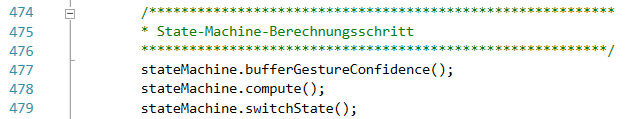
\includegraphics[width=.8\textwidth]{pictures/statemachine-ber.png}
\caption{Der Code, der den Berechnungsschritt der State-Machine darstellt.}\label{fig:ber}
\end{figure}
Am Ende der \texttt{run()}-Methode wird der Frame \glqq{}releast\grqq{} und die bei \texttt{compute()} berechneten \texttt{motionParameters} zurückgegeben. Wie genau sie schließlich verwendet werden, entscheidet das unterliegende Programm.

	\subsection{Einbinden}\label{sec:einbinden}
Das vorliegende Projekt kompiliert eine statische Bibliothek (.lib). Diese ist (in Visual Studio) als \glqq{}Additional Dependency\grqq{} für das Linking einzutragen.\par\medskip
Das Programm, das die Library verwendet, sollte mittels \[\texttt{KinectControl kinectControl;}\]ein KinectControl-Objekt anlegen und in seiner Initialisierung durch Aufruf seiner \texttt{init()}-Funktion mitinitialisieren: \[\texttt{kinectControl.init(this);}\] Dabei wird ein \texttt{ControlWidget} übergeben, für welches die Funktionen \texttt{pickModel()} für die Objektwahl sowie \texttt{sendEvent()} für das Versenden von Nachrichten implementiert sein müssen.\par
Im Main-Loop oder Event-Loop des Programms werden per \[\texttt{MotionParameters motionParameters = kinectControl.run();}\] die Parameter (Translation, Rotation und Ziel) geholt und können ausgewertet und entsprechen angewendet werden.\par 
Weiterhin sollte \texttt{kinectControl.assignMaster()} irgendwie angestoßen werden können, z.\,B. über ein bestimmtes Tastendruck-Event.
%
%
\clearpage
\section{Schlussbemerkungen}
In diesem Abschnitt wollen wir zum Abschluss einserseits feststellen, wie gut die im Projektseminar erstellte Anwendung den für sie vorgesehenen Zweck erfüllt, andererseits aber auch bemerken, wie sich die Kinect selbst überhaupt für eine solche Aufgabe eignet.\par 
Wir geben Ausblick auf sinnvolle und nützliche Erweiterungen der Software und schließen mit einer Gesamtbewertung des Projektes aus unserer Sicht.
%
%
\subsection{Eignung unserer Software}
Die im Projektseminar erstellte Software erfüllt die Aufgabenstellung in einem zufriedenstellenden Maße. Es ist möglich, die 3D-Szene und enthaltene Objekte per Geste zu steuern und diese Steuerung ist (in den Augen der Projektteilnehmer) intuitiv und technisch einfach durchzuführen. Die Steuerung arbeitet relativ präzise, zeigt jedoch in Teilen auch die Störanfälligkeit der Kinect auf. Bei schlechten Daten kann so dennoch ein für den Anwender ärgerliches Zittern oder Wegspringen auftreten. Wir halten den Nutzer daher dazu an, der Kinect im Rahmen seiner Möglichkeiten entgegenzukommen, d.\,h. zum Beispiel keine zu weite Kleidung (offene Jacken) zu tragen und die Hände bei der Steuerung vorzugsweise neben (nicht vor) dem Körper zu haben. Bei der einhändige Objektrotation ist der Einfluss der Kinectgüte am besten erkennbar, vor allem beim Kippen nach vorne bzw. hinten.\par 
Die Mastererkennung funktioniert ebenfalls wie vorgesehen, es kann jedoch im ungünstigsten Falle passieren, dass für den Master ein fehlerhaftes Skelett mit falschen Proportionen beobachtet wird. Dann wird er gegebenenfalls nicht wiedererkannt und das Programm muss neu gestartet werden, um wieder steuerbar zu sein.
%
\subsection{Eignung der Kinect}
Die Kinect eignet sich nur mit Einschränkung für eine sehr präzise $1$"=zu"=$1$"=Abbildung einer Steuerung. Man darf dabei jedoch nicht außer Acht lassen, welcher Herkunft sie ist und dass eine solche Verwendung nicht ihrem vorgesehenen Anwendungsspektrum angehört. Es wäre definitiv einfacher, eine Steuerung durch diskrete Gestenerkennung ohne $1$"=zu"=$1$"=Zusammenhang zu gestalten, bspw. so, dass eine bestimmte Geste eine Bewegung vordefinierter Distanz in eine der Achsenrichtungen bewirkt. Demgegenüber treten bei der Direktabbildung Probleme mit den qualtitativ (wenigstens im Vergleich zu industriell verwendeter Sensortechnik) schlechten bis sehr schlechten Kinectdaten auf. Trotz starker Glättung ist es uns nicht gelungen, den Jitter unter Erhalt der Echtzeitabbildung vollständig zu eliminieren. Auch mit Parameteroptimierung ist an dieser Stelle vermutlich nicht mehr viel zu erreichen.\par 
Bei der Mastererkennung ist die größte Problematik die im vorangegangenen Abschnitt genannte. Dazu kommt, dass es mit unserer Methode schwierig sein könnte, sehr ähnliche Personen zu differenzieren -- wobei bessere Systeme z.\,B. bei der Präsentation eineiiger Zwillinge vermutlich auch an ihre Grenzen kommen. Hierzu hatten wir doch keinen Zugriff auf passende Testpersonen. Mit größerem Aufwand lassen sich jedoch bessere Erkennungsquoten erzielen, vergleiche dazu etwa \cite{appearance}, \cite{biomid} und \cite{bodyprop}. Es gibt auch gänzlich andere Ansätze, wie etwa über den Gang (siehe \cite{gait}) oder das Gesicht (siehe \cite{face}).Selbstverständlich sind die sichersten Erkennungen nicht mehr echtzeitfähig.\par 
Wir schließen an dieser Stelle damit, dass die Kinect für den gegebenen Zweck verwendet werden kann, aber in ihrer Qualität nicht ohne Weiteres an Hochleistungssysteme heranreicht. Gerade zu sicherheitsrelevanten Aufgaben sollte man also nicht am Trackingsystem sparen.
%
\subsection{Verbesserungen}
Obwohl die Kernaufgabenstellung hinlänglich erfüllt ist, möchten wir Ausblick auf potenzielle Verbesserungen unserer Software geben.\par
Zunächst wäre es in der Zukunft natürlich wünschenswert, wenn sämtliche Stubfunktiononalität und der geplante Funktionsumfang implementiert würden, sobald das einbindende Grundprogramm sie unterstützt.\par 
Die Parameter des Programms ließen sich in der Zukunft weiter optimieren. Eventuell sind dafür auch Tests in einem größerem Rahmen -- z.\,B. mit etwa 50 Testpersonen -- nützlich. Diese würden den zusätzlichen Zweck erfüllen, einen besseren Einblick in die Unterschiede zwischen verschiedenen Skeletten zu gewinnen und so bspw. neue Körpermerkmale für die Erkennung zu gewinnen oder weniger aussagekräftige auszusondern.\par 
In der Hinsicht auf Programmparameter währen für den Anwender auch zusätzliche Schnittstellen nach außen wünschenswert, z.\,B. um die Genauigkeit der Mastererkennung von außen vorgeben zu können. Gerade vor diesem Hintergrund war während der Arbeit im Gespräch die Mastererkennung so zu gestalten, dass die Einspeicherung so lange fortwährt, bis die Standardabweichung aller gesammelten Daten unter eine vorgegebene Konvergenzschranke gerät und die erlaubte Abweichung damit anstelle der empirischen Feststellung präzise vorgegeben werden kann. Diese Stoßrichtung wurde aus Zeitgründen in der Arbeitsphase des Projektes verworfen. Insbesondere wäre dies nicht ohne Feedback für den Nutzer sinnvoll, da dieser sonst über keinerlei Wissen verfügt, wie lange die Masterfestlegung (noch) dauern wird. Daher sollte vor dieser Implementierung ein komplett funktionstüchtiges Eventsystem bereitstehen und von der Grundanwendung eine Ausgabemöglichkeit gegeben sein.\par 
Darüber hinaus gibt es Erweiterungen der Funktionalität, die die Bedienerfahrung verbessern würden. Dies betrifft etwa ein Zurücksetzen des Masters, um die Steuerung abgeben zu können; ein Zurücksetzen von Kamera und Objekten, ggf. per Geste; die Skalierung und das Löschen von Objekten mittels Gesten und sicher viele weitere. Einige solcher Wunschfunktionalitäten ergeben sich erst im Laufe der tatsächlichen Verwendung der Software, wie es etwa bei der hinzugekommenen Aufgabe, einen Flugmodus zu implementieren der Fall war.
%
\subsection{Fazit}
Trotz der Probleme der Kinect, sind wir davon überzeugt, dass unser Programm mit vertretbarem Aufwand eine verwertbare Softwarelösung der Aufgabenstellung darstellt und sie insbesondere für Präsentationen wie an einem Tag der offenen Tür einen Mehrwert darstellt.\par 
Sofern hohe Genauigkeit notwendig ist oder die Anwendung irgendwelchen Sicherheitskriterien genügen muss, empfehlen wir jedoch die Nutzung eines höherwertigen Trackingsystems zuungunsten der Kinect.\par 
Die Arbeit mit der Kinect und mit den Konzepten Gestensteuerung und Personenerkennung war für alle Projektteilnehmer eine wertvolle Erfahrung und abseits der üblichen Schwierigkeiten, die eine solche Projektsituation mit sich zieht, ein reizvolles und erfüllendes Unterfangen.\par\bigskip
Wir möchten abschließend dem Fachgebiet Graphische Datenverarbeitung für die zur Verfügung gesellte Technik nebst Leihmöglichkeit danken und insbesondere unseren Betreuer, Herrn M.\,sc. Julian Meder hervorheben, der zahlreiche Gedanken und Anregungen in das Projekt einfließen lies, kreativ in seinen Vorstellungen vom Funktionsumfang des Programmes war und unsere Fragen stets zügig und kompetent beantwortete.
%TODO verwendete Werkzeuge

\newpage
\nocite{*}
\printbibliography
\end{document}